% Template for PLoS
% Version 3.5 March 2018
%
% % % % % % % % % % % % % % % % % % % % % %
%
% -- IMPORTANT NOTE
%
% This template contains comments intended 
% to minimize problems and delays during our production 
% process. Please follow the template instructions
% whenever possible.
%
% % % % % % % % % % % % % % % % % % % % % % % 
%
% Once your paper is accepted for publication, 
% PLEASE REMOVE ALL TRACKED CHANGES in this file 
% and leave only the final text of your manuscript. 
% PLOS recommends the use of latexdiff to track changes during review, as this will help to maintain a clean tex file.
% Visit https://www.ctan.org/pkg/latexdiff?lang=en for info or contact us at latex@plos.org.
%
%
% There are no restrictions on package use within the LaTeX files except that 
% no packages listed in the template may be deleted.
%
% Please do not include colors or graphics in the text.
%
% The manuscript LaTeX source should be contained within a single file (do not use \input, \externaldocument, or similar commands).
%
% % % % % % % % % % % % % % % % % % % % % % %
%
% -- FIGURES AND TABLES
%
% Please include tables/figure captions directly after the paragraph where they are first cited in the text.
%
% DO NOT INCLUDE GRAPHICS IN YOUR MANUSCRIPT
% - Figures should be uploaded separately from your manuscript file. 
% - Figures generated using LaTeX should be extracted and removed from the PDF before submission. 
% - Figures containing multiple panels/subfigures must be combined into one image file before submission.
% For figure citations, please use "Fig" instead of "Figure".
% See http://journals.plos.org/plosone/s/figures for PLOS figure guidelines.
%
% Tables should be cell-based and may not contain:
% - spacing/line breaks within cells to alter layout or alignment
% - do not nest tabular environments (no tabular environments within tabular environments)
% - no graphics or colored text (cell background color/shading OK)
% See http://journals.plos.org/plosone/s/tables for table guidelines.
%
% For tables that exceed the width of the text column, use the adjustwidth environment as illustrated in the example table in text below.
%
% % % % % % % % % % % % % % % % % % % % % % % %
%
% -- EQUATIONS, MATH SYMBOLS, SUBSCRIPTS, AND SUPERSCRIPTS
%
% IMPORTANT
% Below are a few tips to help format your equations and other special characters according to our specifications. For more tips to help reduce the possibility of formatting errors during conversion, please see our LaTeX guidelines at http://journals.plos.org/plosone/s/latex
%
% For inline equations, please be sure to include all portions of an equation in the math environment.  For example, x$^2$ is incorrect; this should be formatted as $x^2$ (or $\mathrm{x}^2$ if the romanized font is desired).
%
% Do not include text that is not math in the math environment. For example, CO2 should be written as CO\textsubscript{2} instead of CO$_2$.
%
% Please add line breaks to long display equations when possible in order to fit size of the column. 
%
% For inline equations, please do not include punctuation (commas, etc) within the math environment unless this is part of the equation.
%
% When adding superscript or subscripts outside of brackets/braces, please group using {}.  For example, change "[U(D,E,\gamma)]^2" to "{[U(D,E,\gamma)]}^2". 
%
% Do not use \cal for caligraphic font.  Instead, use \mathcal{}
%
% % % % % % % % % % % % % % % % % % % % % % % % 
%
% Please contact latex@plos.org with any questions.
%
% % % % % % % % % % % % % % % % % % % % % % % %

\documentclass[10pt,letterpaper,table]{article}
\usepackage[top=0.85in,left=2.75in,footskip=0.75in]{geometry}

%\usepackage{natbib} % bibliography

\usepackage{setspace}
\usepackage{pgf}
\usepackage{tikz}
\usepackage{bm}
\usepackage{soul}
\usetikzlibrary{bayesnet}

\usepackage{tcolorbox} % for text box

\newtcolorbox[auto counter]{mybox}[2][]{width=\textwidth, colback=gray!10, boxrule=0pt, title=Box~\thetcbcounter: #2, #1}


\usepackage{alltt}

% amsmath and amssymb packages, useful for mathematical formulas and symbols
\usepackage{amsmath,amssymb}

% Use adjustwidth environment to exceed column width (see example table in text)
\usepackage{changepage}

% Use Unicode characters when possible
\usepackage[utf8x]{inputenc}

% textcomp package and marvosym package for additional characters
\usepackage{textcomp,marvosym}

% cite package, to clean up citations in the main text. Do not remove.
\usepackage{cite}

% Use nameref to cite supporting information files (see Supporting Information section for more info)
\usepackage{nameref,hyperref}

% line numbers
\usepackage[right]{lineno}

% ligatures disabled
\usepackage{microtype}
\DisableLigatures[f]{encoding = *, family = * }

% color can be used to apply background shading to table cells only
%\usepackage{xcolor}
%\usepackage[dvipsnames]{xcolor}

% array package and thick rules for tables
\usepackage{array}

% underline
\usepackage{soul}

% create "+" rule type for thick vertical lines
\newcolumntype{+}{!{\vrule width 2pt}}

% create \thickcline for thick horizontal lines of variable length
\newlength\savedwidth
\newcommand\thickcline[1]{%
  \noalign{\global\savedwidth\arrayrulewidth\global\arrayrulewidth 2pt}%
  \cline{#1}%
  \noalign{\vskip\arrayrulewidth}%
  \noalign{\global\arrayrulewidth\savedwidth}%
}

% \thickhline command for thick horizontal lines that span the table
\newcommand\thickhline{\noalign{\global\savedwidth\arrayrulewidth\global\arrayrulewidth 2pt}%
\hline
\noalign{\global\arrayrulewidth\savedwidth}}

% for \paragraph
\usepackage{titlesec}
\titleformat{\paragraph}
{\normalfont\normalsize\itshape}{\theparagraph}{}{}
\titlespacing*{\paragraph}
{0pt} {1ex} {0pt} % 0pt, space before, space after

% Remove comment for double spacing
%\usepackage{setspace} 
%\doublespacing

% Text layout
\raggedright
\setlength{\parindent}{0.5cm}
\textwidth 5.25in 
\textheight 8.75in

% Bold the 'Figure #' in the caption and separate it from the title/caption with a period
% Captions will be left justified
\usepackage[aboveskip=1pt,labelfont=bf,labelsep=period,justification=raggedright,singlelinecheck=off]{caption}
\renewcommand{\figurename}{Fig}

% Use the PLoS provided BiBTeX style
\bibliographystyle{plos2015}

% Remove brackets from numbering in List of References
\makeatletter
\renewcommand{\@biblabel}[1]{\quad#1.}
\makeatother



% Header and Footer with logo
\usepackage{lastpage,fancyhdr,graphicx}
\usepackage{epstopdf}

%\pagestyle{myheadings}
\pagestyle{fancy}
\fancyhf{}
%\setlength{\headheight}{27.023pt}
%\lhead{\includegraphics[width=2.0in]{PLOS-submission.eps}}
\rfoot{\thepage/\pageref{LastPage}}
\renewcommand{\headrulewidth}{0pt}
\renewcommand{\footrule}{\hrule height 2pt \vspace{2mm}}
\fancyheadoffset[L]{2.25in}
\fancyfootoffset[L]{2.25in}
\lfoot{\today}

%% Include all macros below

\newcommand{\lorem}{{\bf LOREM}}
\newcommand{\ipsum}{{\bf IPSUM}}

\newcommand{\alexei}[1]{\textcolor{teal}{{\bf ALEXEI}: {#1}}}

% next 6 lines put a caption on \alltt float
\usepackage{newfloat}
\usepackage{caption}
\DeclareFloatingEnvironment[fileext=frm,placement={!ht},name=example]{example}
\DeclareCaptionSubType*{example}
% \captionsetup[subexample]{name=Example}
% \renewcommand{\thesubexample}{\theexample}

\usepackage{listing}

% graphical options
\usepackage{tcolorbox}
\usepackage{color}
\usepackage{xcolor}

\usepackage{environ}
\makeatletter
\newsavebox{\measure@tikzpicture}
\NewEnviron{scaletikzpicturetowidth}[1]{%
  \def\tikz@width{#1}%
  \def\tikzscale{1}\begin{lrbox}{\measure@tikzpicture}%
  \BODY
  \end{lrbox}%
  \pgfmathparse{#1/\wd\measure@tikzpicture}%
  \edef\tikzscale{\pgfmathresult}%
  \BODY
}
\makeatother\usetikzlibrary{bayesnet}

%% END MACROS SECTION


\begin{document}
\vspace*{0.2in}

%%%%%%%%%%%%%%%%%%%%%%%%%%%%%%%%%%%
% Begin comments
%%%%%%%%%%%%%%%%%%%%%%%%%%%%%%%%%%%

% \textcolor{red}{FKM and KC: Here is our shot at providing a skeleton for this paper. At the moment, the order of sections seems backward, the difference between `Methods' and `Results' seems arbitrary, and we have too many listings in the main text. I think support for model averaging should be put into the supplementary. We need to move a lot of it to the Supplementary.}

% \bigskip

% \textcolor{red}{Methods (in the order the bullet points appear!):}
% \begin{enumerate}
%     \item \textcolor{red}{Right after `Methods', not nested within any subsections: What LPHy and its framework do as a simple inline list; This includes (i) model specification and visualization, (ii) data simulation, (iii) model description as natural narratives, (iv) configuration of inferential analyses;}
%     \item \textcolor{red}{(Subsection) LPhy language features: will introduce basic concepts (PGMs, stochastic nodes, etc) and one-liners examplifying how to define a constant, a stochastic and a deterministic node; data clamping; vectorization;} \textcolor{blue}{From Walter: I strongly recommend to use the LPhy terms in this paper that introduced by Alexei previously: Constants, Random variables, Deterministic variables, Generators. @Fabio, I suggest we need to clarify the terms for readers. In my opinion, "Variable" refers to the LPhy code, may be OK also to a node in PGM, but "Node" only refers to the PGM representation of a variable, which should not be used to describe the code.}
%     \item \textcolor{red}{(Subsection) Short description of GUI and CLI (no screenshots just yet, or maybe pointing to a screenshot/figure in the results section);}
%     \item \textcolor{red}{(Subsection) LPhyToBEAST: short paragraph on interface between LPhy and BEAST 2
%     \item \textcolor{red}{(Subsection) Technical details: it's implemented in Java, built as a Gradle project (@Walter: we want like one to two sentences; it was a lot of work for you, certainly, but it is almost entirely irrelevant to the reader), open-source code that is publicly available} \textcolor{blue}{I presume you meant "2.4 As a Gradle project". I just put everything necessary in main for the 1st version of the draft, so we have something to discuss. These technical details can be moved to Suppl. If you meant Introduction, I think Kylie would be happy to refine it after we have a meeting together.}}
%     \newline
% \end{enumerate}

% \textcolor{red}{Results (in the order the bullet points appear!):}
% \textcolor{green}{AJD: One large figure and 2 paragraphs (keep it short and sharp);}
% \begin{enumerate}
%     \item \textcolor{red}{Box and figure: Show a full script specifying a moderately complex model as a listing, and a screenshot of the GUI. I suggest using the phylodynamic hierarchical model from the tutorial (RSV) I wrote way back when;}
%     \item \textcolor{red}{Describe the data/model text blocks in the script;}
%     \item \textcolor{green}{AJD: Show the graphical representation (probabilistic model representation, visualize these models as factor graphs (implies a Bayesian network), small square nodes -- factors or deterministic transformations) }
%     \item \textcolor{red}{Show the natural text narrative;}
%     \item \textcolor{red}{Describe/discuss simulation and using those simulations for a coverage study; (@Walter: you even generated these figures before, we should put them here and discuss them)} \textcolor{blue}{(From Walter: @Fabio, Kylie and I discussed to use her model validation in Phylonco, which supposes to be more interested. Please let me know, if this is not the case any more.)}
%     \item \textcolor{red}{Show/comment on data clamping, generating an .xml for actually using the model for inference with similar data with BEAST 2.}
%     \newline
% \end{enumerate}


% \textcolor{red}{Discussion (in the order the bullet points appear!):}
% \begin{enumerate}
%     \item \textcolor{red}{One or two paragraphs briefly recapitulating and summarizing what we are doing here;}
%     \item \textcolor{red}{One or two paragraph on what LPhy allows us to do (`advantages' of LPhy) relative to what is out there or not out there, mention .Rev and BEAUTi;}
%     \item \textcolor{red}{One paragraph on what LPhy does NOT allow us to do (`limitations' of LPhy);}
%     \item \textcolor{red}{One paragraph on extensibility, release, tutorials, examples, community use, etc.;}
%     \item \textcolor{red}{One paragraph to wrap it up with future directions.}
%     \newline
% \end{enumerate}

% \clearpage

%%%%%%%%%%%%%%%%%%%%%%%%%%%%%%%%%%%
% End comments
%%%%%%%%%%%%%%%%%%%%%%%%%%%%%%%%%%%


% Title must be 250 characters or less.
\begin{flushleft}
{\Large
\textbf\newline{LinguaPhylo: a probabilistic model specification language for
  reproducible phylogenetic analyses} % Please use "sentence case" for title and headings (capitalize only the first word in a title (or heading), the first word in a subtitle (or subheading), and any proper nouns).
}
\newline
% Insert author names, affiliations and corresponding author email (do not include titles, positions, or degrees).
\\
Alexei J. Drummond\textsuperscript{1,2,3}*,
Kylie Chen\textsuperscript{1,2,3},
F\'{a}bio K. Mendes\textsuperscript{1,4},
Dong Xie\textsuperscript{1,2,3}
\\
\bigskip
\textbf{1} Centre for Computational Evolution, University of Auckland, Auckland, New Zealand
\\
\textbf{2} School of Biological Sciences, University of Auckland, Auckland, New Zealand
\\
\textbf{3} School of Computer Science, University of Auckland, Auckland, New Zealand
\\
\textbf{4} Department of Biology, Washington University in St. Louis, St. Louis, United States
\\
\bigskip

% Insert additional author notes using the symbols described below. Insert symbol callouts after author names as necessary.
% 
% Remove or comment out the author notes below if they aren't used.
%
% Primary Equal Contribution Note

% Use the asterisk to denote corresponding authorship and provide email address in note below.
* a.drummond@auckland.ac.nz

\end{flushleft}

% Please keep the abstract below 300 words
\section*{Abstract}
  Phylogenetic models have become increasingly complex and phylogenetic data sets larger and richer.
  Yet inference tools lack a model specification language that succinctly describes a full phylogenetic analysis independently of implementation details.
  We present a new lightweight and concise model specification language, called `LPhy', that is both human and machine readable.
  `LPhy' is accompanied by a graphical user interface for building models and simulating data using this new language, as well as for creating natural language narratives describing such models.
  These narratives can form the basis of manuscript method sections.
  We also introduce a command-line interface for converting LPhy-specified models into analysis specification files (in XML format) to be used alongside the BEAST2 software platform.
  Together, these tools will clarify the description and reporting of probabilistic models in phylogenetic studies, and improve result reproducibility.


% Please keep the Author Summary between 150 and 200 words
% Use first person. PLOS ONE authors please skip this step. 
% Author Summary not valid for PLOS ONE submissions.   
\section*{Author summary}
  We describe a succinct domain-specific language to accurately specify the details of a phylogenetic model for the purposes of reproducibility or reuse.
  In addition, we have developed a graphical software package that can be used to construct and simulate data from models described in this new language, as well as create natural language narratives that can form the basis of a description of the model for the method section of a manuscript.
  Finally, we report on a command-line program that can be used to generate input files for the BEAST2 software package based on a model specified in this new language.
  These tools together should aid in the goal of reproducibility and reuse of probabilistic phylogenetic models. 


\linenumbers

% Use "Eq" instead of "Equation" for equation citations.
\section{Introduction}

Transparency is a scientific ideal, and replicability and
reproducibility lie at the heart of the scientific endeavor
\cite{nas19,munafo17}. 
Metaresearch efforts have uncovered the so-called ``reproducibility
crisis'' \cite{baker16} in many scientific domains \cite{baker16}. 
In recent years, the growing number of computational biology software packages available has enabled greater choice in data analyses, 
but at the cost of increased complexity in the data-preparation and analytical pipelines \cite{eren2021community}. 
This increases the difficulty of accurately reporting and reproducing analyses. 
These barriers have been recognized by the wider genomics research community \cite{eren2021community} as well as within evolutionary biology \cite{oakley2014osiris}. 

In evolutionary biology, phylogenetics has become a highly technical discipline \cite{oakley2014osiris}. 
The most general phylogenetic tools are Bayesian methods (e.g., BEAST, BEAST 2, MrBayes and
RevBayes; \cite{beast,beast2,revbayes,mrbayes}) 
that can simultaneously reconstruct phylogenetic tree topology and divergence times, as well as estimate the related micro-evolutionary and macro-evolutionary parameters. 
Phylogenetic analyses often combine multiple models within a complex pipeline to answer questions in evolutionary biology such as species evolution \cite{gavryushkina17,ogilvie21,zhang21}, ancestral bio-geographical ranges \cite{lemey10,landis18}, and 
% ecological networks \cite{braga20}, 
% trait evolution \cite{may19,bite}, and 
epidemic dynamics \cite{faria21,douglas21}. 

Reproducing, reusing and interpreting a phylogenetic model is not trivial, and requires an understanding of the input data, details of the model (i.e., its parameters and how they are are related and their priors), and inference methodology. 
The latter can include complex Markov chain Monte Carlo (MCMC) proposal distributions and sampling algorithms which are not part of the model.
Currently, little research has been done on the readability, reproducibility and re-usability of phylogenetic analyses employing phylogenetic models. 
Our paper presents a tool that aims to: (i) facilitate concise communication of phylogenetic models, (ii) improve reproducibility, and (iii) increase re-usability of phylogenetic models and their variations on new datasets. 
 
Previous attempts to address model specification and analysis setup include BEAST-style XMLs (eXtensible Markup Language) developed for the BEAST software \cite{beast,beast2} and the Rev programming language for RevBayes \cite{revbayes}. 
The extensibility of XMLs provides flexibility to developers allowing them to create new descriptive tags for specifying new models.
However, BEAST-style XMLs are hard to read due to their verbose syntax and the usual complexity of the models being specified. 
Unsurprisingly, translating BEAST or BEAST 2 analyses from XMLs into text descriptions is difficult and error prone. Our experience suggests that most users are unable to verify if the XML analysis file matches the description in their manuscript.
The Rev language \cite{revbayes} is an alternative to XMLs, and it incorporates conventional notation from more general probabilistic programming languages. 
This feature makes Rev model specification more recognisable to statistically literate users and sometimes more flexible, but users must still contend with verbose and prosaic implementation 
details extraneous to the model
(such as MCMC sampling settings, logging details and proposal distributions), as well as with the error-prone task of describing the REV model accurately in natural language when describing it in the methods section of a manuscript.
 
Here, we introduce LinguaPhylo (LPhy, pronounced `el-fee'), an open-source model specification 
language aimed at improving readability, reproducibility, and re-usability of phylogenetic models. 
The LPhy language has a simple syntax for succinct specification of complex models, and is implemented in a framework that generates precise text descriptions and graphical diagrams of phylogenetic models from user input.

\section{Methods}
The LPhy language is designed to enable the specification of phylogenetic models using a concise and readable syntax.  
The reference implementation is built on top of the Java programming language and provides features for: 
(i) concise formal specification of phylogenetic models on real or synthetic data, (ii) data simulation from phylogenetic models, (iii) integration with the BEAST 2 phylogenetic inference framework, and (iv) an extensibility mechanism for adding new functionality and data types to the LPhy language.

\subsection{Language features}
The LPhy language provides a simple syntax for specifying and simulating under different evolutionary models models.
These include tree models for phylogenies and genealogies (e.g., birth-death, coalescent), substitution models for genomic sequences (e.g., GTR \cite{gtr}), and parametric distributions for discrete and continuous parameters (e.g., Dirichlet, Normal). 


In the context of simulation under a model specified with LPhy, ``generative distributions'' produce values for random variables, which in turn can be of different ``datatypes'': trees, continuous morphology, sequence alignments.
These random variables constitute stochastic nodes in the probabilistic graphical model (PGM) that LPhy builds, but it is also possible to assign a fixed value to a node, in which case a constant node is created (see more on this below).

% \textcolor{blue}{[FKM: Don't think the following should appear here]}\textcolor{red}{\st{An input API is provided to parse input sequences from nexus and fasta formats and trees from newick format into `LPhy datatypes'. A full list of available distributions and determinisitic functions are shown in the supplementary materials tables S1 - S4.}}

The specification of generators and named variables is done through commands the user can type on LPhy's command prompt or execute from a script file:

{
  \small
  \begin{listing}
    \stepcounter{example}
    \begin{alltt}
  data \{
    L = \textcolor{magenta}{200};
    taxa = \textcolor{magenta!80!black}{taxa}(names=\textcolor{magenta}{1}:\textcolor{magenta}{10});
  \}
  model \{
    \textcolor{green}{\(\Theta\)} ~ \textcolor{blue}{LogNormal}(\textcolor{gray}{meanlog=}\textcolor{magenta}{3.0}, \textcolor{gray}{sdlog=}\textcolor{magenta}{1.0});
    \textcolor{green}{\(\psi\)} ~ \textcolor{blue}{Coalescent}(\textcolor{gray}{theta=}\textcolor{green}{\(\Theta\)}, \textcolor{gray}{taxa=}taxa);
    \textcolor{green}{D} ~ \textcolor{blue}{PhyloCTMC}(\textcolor{gray}{L=}L, \textcolor{gray}{Q=}\textcolor{magenta!80!black}{jukesCantor}(), \textcolor{gray}{tree=}\textcolor{green}{\(\psi\)});
  \}
    \end{alltt}
    \caption{\small{An LPhy script defining a constant-size coalescent tree prior with log-normally distributed population sizes, a strict clock model, and a Jukes-Cantor model on 10 nucleotide sequences with 200 sites (base pairs).}}
    \label{lphy:jccoal}
  \end{listing}
}
% \textcolor{blue}{TODO: cannot change caption from Listing 1 to Example 1.}

\medskip{}

Listing \ref{lphy:jccoal} specifies a complete phylogenetic model using only five lines of code inside two blocks. Constant nodes with fixed values are shown in magenta.  
The first block specifies ``200'' nucleotide sites in ``L'' and ten different taxa named `1' to `10' in ``taxa''. 
The second block declares the stochastic nodes or random variables in green, and their generative distributions in blue.

% \textcolor{red}{\st{The phylogenetic models constructed from the LPhy language are fitting in the probabilistic graphical model framework. Under this framework, the LPhy language introduces four types of components listed below:}}

\begin{figure}
   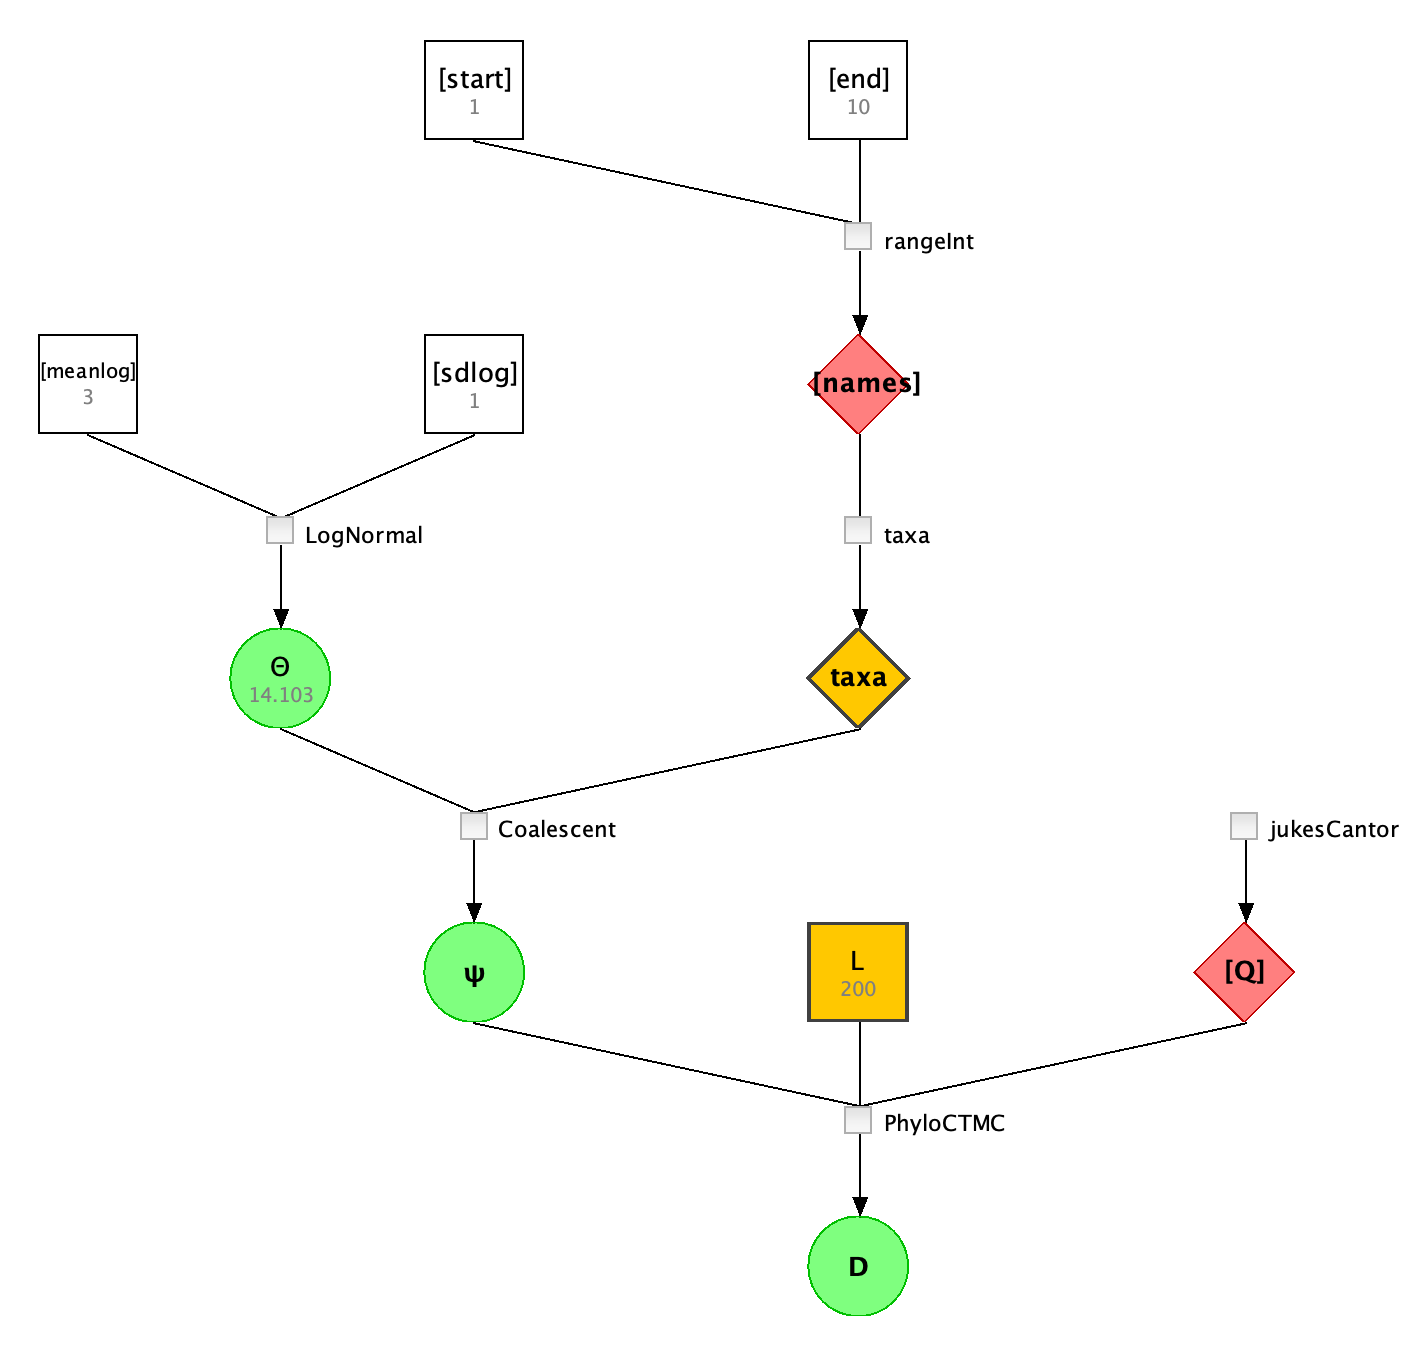
\includegraphics[width=0.8\textwidth]{figs_plos/jc_coal.png}
  \caption{The graphical representation of the probabilistic model defined in Listing \ref{lphy:jccoal}.} 
  \label{fig:jccoalPGM}
\end{figure}

% \begin{itemize}
%     \item \textcolor{red}{\st{Constants;}}
%     \item \textcolor{red}{\st{Random variables;}}
%     \item \textcolor{red}{\st{Deterministic variables;}}
%     \item \textcolor{red}{\st{Generators: generative distribution, function, and method call.}}
% \end{itemize}

There are three classes of generators: (i) generative distrivutions which produce values for random variables, (ii) deterministic functions, and (iii) method calls.
%In addition to producing values for random variables, where the generators are generative distributions, two other classes of generators are deterministic functions and method calls.
For deterministic functions and method calls, these generators produce deterministic nodes in the PGM.
This is illustrated in Figure \ref{fig:jccoalPGM}, which shows a graphical representation of the model specified in Listing \ref{lphy:jccoal}.
Deterministic nodes are shown as diamonds (e.g., the ``Q'' matrix of the Jukes-Cantor model).
Stochastic nodes are represented by circles (e.g., $\Theta$, the population size governing the coalescent times generated by the Coalescent process), and constant nodes are represented by squares (e.g., the mean of the log-normal generative distribution underlying $\Theta$).

% \textcolor{red}{\st{As it can be seen in Figure \ref{fig:jccoalPGM}, the constants are drawn as the big squares, whose values are fixed, such as the mean or stand deviation for a probabilistic distribution, file name, and so on.}}

% \textcolor{red}{\st{The random variables contain the values generated from generative distributions, and they are also the set of parameters to estimate in the specified phylogenetic model. They are drawn as the green circles. But when there is an observed data clamped into a random variable (Section \ref{sec:dataclamping}) to replace its previous value, such as importing an alignment, the circle representing it will be coloured by blue.}}

% \textcolor{red}{\st{The values of deterministic variables can be generated from either deterministic functions or method calls, but their values will be fixed when given the same inputs to their generators. They are drawn as diamonds. If the value is generated inside the data block, then it will be coloured by yellow, otherwise it will be a red diamond.}}

% \textcolor{red}{\st{Generative distributions, (deterministic) functions and method calls are all the generators. They are drawn as the small boxes.}}

\subsubsection{Variable vectorization}

Named variables in LPhy can be scalars or vectors. Any generator can be vectorized to produce a vector of i.i.d. values by using the \texttt{replicates} keyword:

{\small
\begin{alltt}
    \textcolor{green}{\(\kappa\)} ~ \textcolor{blue}{LogNormal}(\textcolor{gray}{meanlog=}\textcolor{magenta}{0.5}, \textcolor{gray}{sdlog=}\textcolor{magenta}{1.0}, \textcolor{gray}{replicates=}\textcolor{magenta}{3});
\end{alltt}
}

Vectorization can also be applied to a generative distribution that already produces vectors. In which case, the output will be a matrix as in the following example, where the major dimension has size 3, with each element of the $\pi$ random variable being a vector of base frequencies.

{\small
\begin{alltt}
      \textcolor{green}{\(\pi\)} ~ \textcolor{blue}{Dirichlet}(\textcolor{gray}{conc=}[\textcolor{magenta}{2.0}, \textcolor{magenta}{2.0}, \textcolor{magenta}{2.0}, \textcolor{magenta}{2.0}], \textcolor{gray}{replicates=}\textcolor{magenta}{3});
\end{alltt}
}

% The first line of the following code is another example of using IID to sample three sets of base frequencies for the three-partition model. 
% Combining with the above line, the second line below vectorises the \texttt{hky} function by passing arguments that are arrays themselves (i.e. \texttt{$\kappa$} and \texttt{$\pi$}).
In the example above, $\kappa$ is a random vector of three log-normally distributed i.i.d. values. 

Finally, vectorization can be coerced simply by passing a vector input instead of a scalar input to one or more of the inputs of a generator:

{\small
\begin{alltt}
    \textcolor{black}{Q = }\textcolor{magenta!80!black}{hky}(\textcolor{gray}{kappa=}\textcolor{green}{\(\kappa\)}, \textcolor{gray}{freq=}\textcolor{green}{\(\pi\)});
\end{alltt} 
}

Here, since both $\kappa$ and $\pi$ are random vectors with the same major dimension length (3), we can assign them as values of the \texttt{hky} deterministic function, which in turn outputs a vector of three instantaneous rate matrices, stored in $Q$.

% Examples below
\subsubsection{Parametric distributions}
LPhy implements a series of parametric distributions commonly used in evolutionary models, such as Uniform, Normal, Lognormal, Gamma, Exponential, and Dirichlet. 
Specifying parametric distributions as generative distributions for model parameters can be achieved by:

%and $\Theta$. 
%Here, $\mu$ is generated from a LogNormal distribution with a mean of $-5$ and a standard deviation of $1.25$. 
%The variable $\Theta$ is generated from a LogNormal distribution with a mean of $3.0$ and a standard deviation of $2.0$.  

{\small
\begin{alltt}
    \textcolor{green}{\(\mu\)} ~ \textcolor{blue}{LogNormal}(\textcolor{gray}{meanlog=}\textcolor{magenta}{-5.0}, \textcolor{gray}{sdlog=}\textcolor{magenta}{1.25});
\end{alltt}}

Each parametric distribution is characterized by its own parameters. 
In the example above, the extinction rate parameter $\mu$ is drawn from a Lognormal distribution with mean -5 and standard deviation 1.25 in log space.
%  \textcolor{green}{\(\Theta\)} ~ \textcolor{blue}{LogNormal}(\textcolor{gray}{meanlog=}\textcolor{magenta}{3.0}, \textcolor{gray}{sdlog=}\textcolor{magenta}{2.0});

\subsubsection{Tree models}
\label{sec:treeprior}
Tree models are central components in phylogenetic simulation and analysis, and are used to generate phylogenetic trees. Below we briefly expand on some of the main tree models implemented in LPhy.
\newline

\noindent \textbf{Coalescent models}
\paragraph{Serially sampled coalescent}
The simplest coalescent model LPhy implements is the constant-population size coalescent, which can be extended to generate serially sampled (heterochronous) data \cite{Rodrigo1999SerialCoalescent}:
{\small
  \begin{alltt}
    \textcolor{green}{\(\psi\)} ~ \textcolor{blue}{Coalescent}(\textcolor{gray}{theta=}\textcolor{green}{\(\Theta\)}, \textcolor{gray}{taxa=}\textcolor{magenta!80!black}{taxa}(\textcolor{gray}{names=}[\textcolor{magenta}{"a"}, \textcolor{magenta}{"b"}, \textcolor{magenta}{"c"}, \textcolor{magenta}{"d"}], 
      \textcolor{gray}{ages=}[\textcolor{magenta}{0.0}, \textcolor{magenta}{1.0}, \textcolor{magenta}{2.0}, \textcolor{magenta}{3.0}]));
  \end{alltt}
}

The script above specifies a serially sampled constant-population size coalescent (a generative distribution) for tree $\psi$ with four taxa, -- ``a'', ``b'', ``c'', and ``d'' -- sampled at 0.0, 1.0, 2.0 and 3.0 time points, respectively. Here, sample time is defined as the age of a sample, with 0.0 meaning the present moment.

\paragraph{Structured coalescent}
The structured coalescent \cite{hudson1990oxford, notohara1990coalescent} generalizes the constant-population size coalescent \cite{kingman82} by allowing multiple demes, each of which are characterized by a distinct population size (in the simplest case this population size does not change through time).
Demes exchange individuals according to migration rates $m$ specified in the off-diagonal elements of a migration matrix $M$, where the diagonal elements store the population sizes, $\theta$, of each deme.
For $K$ demes, the population size parameter ``theta'' is a $K$-tuple, and $m$ is a $(K^2-K)$-tuple.

{\small
  \begin{alltt}
    M = \textcolor{magenta!80!black}{migrationMatrix}(\textcolor{gray}{theta}=[\textcolor{magenta}{0.1}, \textcolor{magenta}{0.1}], \textcolor{gray}{m}=[\textcolor{magenta}{1.0}, \textcolor{magenta}{1.0}]);
    \textcolor{green}{g} ~ \textcolor{blue}{StructuredCoalescent}(\textcolor{gray}{M}=M, \textcolor{gray}{n}=[\textcolor{magenta}{15}, \textcolor{magenta}{15}]);
  \end{alltt}
}

In the above, \texttt{migrationMatrix} is a deterministic function and \texttt{StructuredCoalescent} is a generative distribution; both are generators. A stochastic node ``g'' stores a gene tree sampled from a two-deme structured coalescent process.

\paragraph{Skyline coalescent model}
The skyline coalescent model \cite{drummond2005bayesian} is a coalescent process that models changes in population sizes.
This model is characterized having a constant population size for each coalescent interval, with instantaneous changes in population size at some coalescent events.

The following script specifies a Skyline coalescent model with 10 coalescent intervals (hence 11 taxa), governed by four distinct population sizes.

{\small
  \begin{alltt}
    \textcolor{green}{g} ~ \textcolor{blue}{SkylineCoalescent}(\textcolor{gray}{theta}=[\textcolor{magenta}{0.1}, \textcolor{magenta}{0.2}, \textcolor{magenta}{0.3}, \textcolor{magenta}{0.4}], \textcolor{gray}{groupSizes}=[\textcolor{magenta}{4},\textcolor{magenta}{3},\textcolor{magenta}{2},\textcolor{magenta}{1}]);
  \end{alltt}
}

Here, ``g'' is a stochastic node in the PGM, with its value sampled from the \texttt{SkylineCoalescent} generative distribution. Ten coalescent intervals are defined through the ``groupSizes'' argument: the first four coalescent intervals will be drawn assuming a ``theta'' of 0.1, the next three intervals with ``theta'' equal to 0.2, and so on.
\newline

\noindent \textbf{Birth-death models}

Birth-death models are commonly used in macroevolution as sampling distributions for species trees. Models that parameterize the fossilization process can be especially useful, as they allow users to leverage fossil ages as data; when fossil morphological characters have also been scored, total-evidence dating can be carried out \cite{ogilvie21}. One such tree model is the serially sampled birth-death process \cite{stadler2013dating}, whose parameters ``psi'' and ``rho'' (see below) represent the rate of sampling extinct and extant lineages, respectively:
% Now leaves of the tree can either be extinct (psi-sampled) or extant (rho-sampled).

{\small
  \begin{alltt}
    ages = [\textcolor{magenta}{0.0}, \textcolor{magenta}{1.0}, \textcolor{magenta}{2.0}, \textcolor{magenta}{3.0}, \textcolor{magenta}{4.0}];
    \textcolor{green}{tree} ~ \textcolor{blue}{BirthDeathSerialSampling}(\textcolor{gray}{lambda}=1, \textcolor{gray}{mu}=\textcolor{magenta}{0.5}, \textcolor{gray}{rho}=\textcolor{magenta}{0.1},
    \textcolor{gray}{psi}=\textcolor{magenta}{1}, \textcolor{gray}{rootAge}=\textcolor{magenta}{5}, \textcolor{gray}{ages}=ages);
  \end{alltt}
}

Other tree models include the birth-death \cite{kendall1948generalized} and fossilized birth-death processes \cite{heath2014fossilized}, as well as the Yule process \cite{yule1925ii}. See the Supplementary Material for more examples.

% \textcolor{blue}{TODO: Shall we add 1. FDB; 2. examples/totalEvidence.lphy}
% FBD and total evidence examples to go in supplementary


\subsubsection{Substitution models}
Substitution models consist of continuous-time Markov chains (CTMC) used to model the evolution of discrete characters, such as nucleotides and amino acid residues. 
LPhy implements a general formulation of a phylogenetic CTMC, known as the GTR model \cite{gtr}, under which several nested models can be specified. 
The first line below constructs the instantaneous rate matrix (Q) for an HKY model \cite{hasegawa1985dating}, which is then used to in \texttt{PhyloCTMC}, the generative distribution over sequence alignment data (D):

{
  \small
  \begin{listing}
    \stepcounter{example}
    \begin{alltt}
    Q = \textcolor{magenta!80!black}{hky}(\textcolor{gray}{kappa}=\textcolor{magenta}{2.0}, \textcolor{gray}{freq}=[\textcolor{magenta}{0.2}, \textcolor{magenta}{0.25}, \textcolor{magenta}{0.3}, \textcolor{magenta}{0.25}]);
    \textcolor{green}{\(\Theta\)} ~ \textcolor{blue}{LogNormal}(\textcolor{gray}{meanlog=}\textcolor{magenta}{3.0}, \textcolor{gray}{sdlog=}\textcolor{magenta}{1.0});
    \textcolor{green}{\(\psi\)} ~ \textcolor{blue}{Coalescent}(\textcolor{gray}{theta=}\textcolor{green}{\(\Theta\)}, \textcolor{gray}{taxa=}taxa);
    \textcolor{green}{D} ~ \textcolor{blue}{PhyloCTMC}(\textcolor{gray}{L=}\textcolor{magenta}{200}, \textcolor{gray}{Q=}Q, \textcolor{gray}{tree=}\textcolor{green}{\(\psi\)});
    \end{alltt}
  \end{listing}
}

Other substitution models can be easily specified by assigning different instantaneous transition rate (Q) matrices to \texttt{PhyloCTMC}, e.g., the matrix of the Jukes-Cantor model \cite{jc69}:
{
  \small
  \begin{listing}
    \stepcounter{example}
    \begin{alltt}
    \textcolor{green}{D} ~ \textcolor{blue}{PhyloCTMC}(\textcolor{gray}{L=}\textcolor{magenta}{200}, \textcolor{gray}{Q=}\textcolor{magenta!80!black}{jukesCantor}(), \textcolor{gray}{tree=}\textcolor{green}{\(\psi\)});
    \end{alltt}
  \end{listing}
}

For forward simulation \texttt{PhyloCTMC} is used as a generative distribution for a multiple sequence alignment, which is here represented by stochastic node ``D''. When the model is employed for statistical inference, and data D is known, the \texttt{PhyloCTMC} represents the phylogenetic likelihood (see Data clamping below).

\subsubsection{Evolutionary clock models}
\label{sec:clockmodels}

Evolutionary (molecular) clock models are used to model the rate of evolutionary change and whether/how it varies over time. The LPhy language supports strict \cite{zuckerkandl1965evolutionary, zuckerkandl1965molecules}, local \cite{drummond2010bayesian} and relaxed clock \cite{drummond2006relaxedconfidence} models. 
Specifying a clock model is done by generating evolutionary rate values, one per phylogenetic tree branch, and then multiplying those rates by the length of the corresponding branch (measured in the chosen units of time) -- effectively scaling the tree to units of expected substitutions per site. 

The simplest clock model is the strict clock, under which the evolutionary rate remains constant over the entire tree. Specifying a strict molecular clock can be done by specifying the ``mu'' parameter in the \texttt{PhyloCTMC} distribution (default is 1.0):
{\small
\begin{alltt}
    \textcolor{green}{\(\lambda\)} ~ \textcolor{blue}{LogNormal}(\textcolor{gray}{meanlog=}\textcolor{magenta}{3.0}, \textcolor{gray}{sdlog=}\textcolor{magenta}{1.0});
    \textcolor{green}{\(\psi\)} ~ \textcolor{blue}{Yule}(\textcolor{gray}{lambda=}\textcolor{green}{\(\lambda\)}, \textcolor{gray}{n=}\textcolor{magenta}{16});
    \textcolor{green}{D} ~ \textcolor{blue}{PhyloCTMC}(\textcolor{gray}{L=}\textcolor{magenta}{200}, \textcolor{gray}{Q=}\textcolor{magenta!80!black}{jukesCantor}(), \textcolor{gray}{tree=}\textcolor{green}{\(\psi\)}, \textcolor{gray}{mu=}\textcolor{magenta}{0.5});
\end{alltt}
}
% [INSERT EXAMPLE HERE WHERE A TREE IS FIRST ASSIGNED A GENERATIVE DISTRIBUTION LIKE THE YULE, AND THEN THAT TREE IS USED IN THE PHYLOCTMC]
% \newline
% \newline
More realistic clock models like the uncorrelated relaxed clock model \cite{drummond2006relaxedconfidence} assume the rate for each branch is drawn according to a parametric distribution. For example, a relaxed clock with rates drawn from a log-normal distribution can be constructed as follows:

{
\small
\begin{alltt}
  \textcolor{green}{\(\lambda\)} ~ \textcolor{blue}{LogNormal}(\textcolor{gray}{meanlog=}\textcolor{magenta}{3.0}, \textcolor{gray}{sdlog=}\textcolor{magenta}{1.0});
  \textcolor{green}{\(\psi\)} ~ \textcolor{blue}{Yule}(\textcolor{gray}{lambda=}\textcolor{green}{\(\lambda\)}, \textcolor{gray}{n=}\textcolor{magenta}{16});
  \textcolor{green}{branchRates} ~ \textcolor{blue}{LogNormal}(\textcolor{gray}{sdlog=}\textcolor{magenta}{0.5}, \textcolor{gray}{meanlog=}\textcolor{magenta}{-0.25}, \textcolor{gray}{replicates=}\textcolor{green}{\(\psi\)}.\textcolor{magenta!80!black}{branchCount}());
  \textcolor{green}{D} ~ \textcolor{blue}{PhyloCTMC}(\textcolor{gray}{L=}\textcolor{magenta}{200}, \textcolor{gray}{Q=}\textcolor{magenta!80!black}{jukesCantor}(), \textcolor{gray}{branchRates=}\textcolor{green}{branchRates}, \textcolor{gray}{tree=}\textcolor{green}{\(\psi\)});
\end{alltt}
}
% {\small
% \begin{alltt}
%     \textcolor{green}{branchRates} ~ \textcolor{blue}{LogNormal}(\textcolor{gray}{meanlog=}\textcolor{magenta}{0.5}, \textcolor{gray}{sdlog=}\textcolor{magenta}{-0.25}, \textcolor{gray}{replicates=}\textcolor{magenta}{30});
% \end{alltt}
% }
% \newline
% [NEED TO SHOW IN THE EXAMPLE ABOVE HOW TO USE ``branchRates'', THAT IS, HOW TO SCALE THE TREE -- AND THEN USE THE SCALED TREE INSIDE PHYLOCTMC. SOMEONE PLEASE UPDATE/FIX THIS EXAMPLE SCRIPT]
% \newline

Here, 30 rates are drawn independently from a log-normal distribution, and then each is assigned to one of the 30 branches of tree $\psi$.

\subsubsection{Inference and data clamping}
\label{sec:dataclamping}
In addition to simulation, LPhy allows users to use a specified model for inference (at the moment, LPhy interfaces only with BEAST 2, see the ``LPhy and BEAST 2'' section below). The key step when setting up an inferential analysis with LPhy, after specifying the model, is to carry out ``data clamping''.

Data clamping should be familiar to users of the Rev language \cite{revbayes}, and consists of assigning an observed value to a random variable in the probabilistic model (i.e., to a stochastic node in the PGM). Effectively, by clamping data to a node, a user tells the inference machinery that the value of a random variable is known and will be conditioned on for purposes of inference. In LPhy, data clamping can be achieved using the ``data block", for example:

% rsv2 example
{
  \small
  \begin{listing}
    \stepcounter{example}
    \begin{alltt}
      data \{
      \quad options = \{\textcolor{gray}{ageDirection=}\textcolor{magenta}{"forward"}, \textcolor{gray}{ageRegex=}\textcolor{magenta}{"s(\textbackslash{}d+)"}\};
      \quad nexusFilePath = \textcolor{magenta}{"tutorials/data/RSV2.nex"};
      \quad D = \textcolor{magenta!80!black}{readNexus}(\textcolor{gray}{file=}nexusFilePath, \textcolor{gray}{options=}options);
      \quad codon = D.\textcolor{magenta!80!black}{charset}([\textcolor{magenta}{"3-629\textbackslash{}3"}, \textcolor{magenta}{"1-629\textbackslash{}3"}, \textcolor{magenta}{"2-629\textbackslash{}3"}]);
      \quad n = \textcolor{magenta}{3};
      \quad L = [\textcolor{magenta}{209}, \textcolor{magenta}{210}, \textcolor{magenta}{210}];
      \quad taxa = D.\textcolor{magenta!80!black}{taxa}();
      \}
      model \{
      \quad \textcolor{green}{\(\pi\)} \textasciitilde \textcolor{blue}{Dirichlet}(\textcolor{gray}{replicates=}n, \textcolor{gray}{conc=}[\textcolor{magenta}{2.0}, \textcolor{magenta}{2.0}, \textcolor{magenta}{2.0}, \textcolor{magenta}{2.0}]);
      \quad \textcolor{green}{\(\kappa\)} ~ \textcolor{blue}{LogNormal}(\textcolor{gray}{sdlog=}\textcolor{magenta}{0.5}, \textcolor{gray}{meanlog=}\textcolor{magenta}{1.0}, \textcolor{gray}{replicates=}n);
      \quad \textcolor{green}{r} ~ \textcolor{blue}{WeightedDirichlet}(\textcolor{gray}{conc=}\textcolor{magenta!80!black}{rep}(\textcolor{gray}{element=}\textcolor{magenta}{1.0}, \textcolor{gray}{times=}n), \textcolor{gray}{weights=}L);
      \quad \textcolor{green}{\(\mu\)} ~ \textcolor{blue}{LogNormal}(\textcolor{gray}{meanlog=}\textcolor{magenta}{-5.0}, \textcolor{gray}{sdlog=}\textcolor{magenta}{1.25});
      \quad \textcolor{green}{\(\Theta\)} ~ \textcolor{blue}{LogNormal}(\textcolor{gray}{meanlog=}\textcolor{magenta}{3.0}, \textcolor{gray}{sdlog=}\textcolor{magenta}{2.0});
      \quad \textcolor{green}{\(\psi\)} ~ \textcolor{blue}{Coalescent}(\textcolor{gray}{taxa=}taxa, \textcolor{gray}{theta=}\textcolor{green}{\(\Theta\)});
      \quad Q = \textcolor{magenta!80!black}{hky}(\textcolor{gray}{kappa=}\textcolor{green}{\(\kappa\)}, \textcolor{gray}{freq=}\textcolor{green}{\(\pi\)}, \textcolor{gray}{meanRate=}\textcolor{green}{r});
      \quad \textcolor{green}{codon} ~ \textcolor{blue}{PhyloCTMC}(\textcolor{gray}{L=}L, \textcolor{gray}{Q=}Q, \textcolor{gray}{mu=}\textcolor{green}{\(\mu\)}, \textcolor{gray}{tree=}\textcolor{green}{\(\psi\)});
      \}
    \end{alltt}
    \caption{An LPhy script for phylodynamic analysis of a virus dataset containing Respiratory syncytial virus subgroup A (RSVA) genomic samples \cite{zlateva2004molecular, zlateva2005genetic}.
    \newline}
    \label{lphy:rsva}
  \end{listing}
}

In the example above, we used a Respiratory syncytial virus subgroup A (RSVA) dataset \cite{zlateva2004molecular, zlateva2005genetic} containing 129 molecular sequences coding for the G protein collected between years 1956 and 2002. 
We use three partitions corresponding to the codon position, an HKY substitution model \cite{hasegawa1985dating}, coalescent tree prior \cite{kingman82} and a strict molecular clock with a Lognormal prior on the mean clock rate. 
Within the \texttt{data} block we clamp the value of ``codon'', a stochastic node that appears below inside the \texttt{model} block. This is achieved by specifying a data node of the same name (codon) in the data block. In this example the data is vectorized into three codon positions to allow different site models for the different codon positions.

% In LPhy language, the alignment is generated by the sampling distribution that the phylogenetic likelihood is derived from, such as a PhyloCTMC generative distribution. The data type of the alignment can be various, for instance, the continuous trait can be simulated from a PhyloBrownian generative distribution. 

% However, in a real data analysis, it requires to pass the imported alignment as an observed state, rather than the simulated alignment to a Bayesian phylogenetic inference engine. So we implement a mechanism called as data clamping for this kind of tasks. 
% The simulated alignment generated by PhyloCTMC in the model block is encapsulated in a random variable mostly in the sink of the probability graph. 
% When the data block has the same random variable containing an existing alignment (e.g. imported from a file), the simulated alignment will be replaced by this imported alignment. 
% This is a useful feature for users to easily switch the task of a LPhy script between simulating alignments and a real data analysis. 

% \textcolor{blue}{TODO: review, and citation multivariate Brownian}

% \subsubsection{\st{Phylogenetic likelihood distributions}}
% \textcolor{blue}{FKM: Not sure if we need this section at all, especially here in the main body. I think we can mention other likelihoods in the Discussion as future directions}
% \st{The phylogenetic continuous-time Markov chain (PhyloCTMC) \cite{felsenstein1981} in the LPhy language is a core generative distribution derived from the phylogenetic likelihood. It takes the other basic models as inputs, such as phylogenetic time tree, instantaneous rate matrix, molecular clock rate, and so on, and on this account simulates a sequence alignment for every leaf node, and also every direct ancestor node when they exist. One example is available in Section \ref{sec:clockmodels}.}

% \st{There are also alternative generative distributions developed in LPhy, which are derived from a different kind of phylogenetic likelihoods, such as the phylogenetic Brownian motion process\cite{felsenstein1973maximum}, its multivariate version, and Ornstein-Ulhenbeck process\cite{felsenstein1973maximum}. Using them, a continuous trait can be simulated from the specified models. For example, running the following LPhy script, the continuous trait $y$ containing 16 continuous values are simulated from a Yule tree $\psi$ with the root value $y0$ sampled from a normal distribution at the diffusion rate $\sigma$ sampled from a log-normal distribution.}

% {\small
% \begin{alltt}
%     \textcolor{green}{\(\lambda\)} ~ \textcolor{blue}{LogNormal}(\textcolor{gray}{meanlog=}\textcolor{magenta}{3.0}, \textcolor{gray}{sdlog=}\textcolor{magenta}{1.0});
%     \textcolor{green}{\(\psi\)} ~ \textcolor{blue}{Yule}(\textcolor{gray}{lambda=}\textcolor{green}{\(\lambda\)}, \textcolor{gray}{n=}\textcolor{magenta}{16});
%     \textcolor{green}{\(\sigma\)} ~ \textcolor{blue}{LogNormal}(\textcolor{gray}{meanlog=}\textcolor{magenta}{1.0}, \textcolor{gray}{sdlog=}\textcolor{magenta}{0.5});
%     \textcolor{green}{y0} ~ \textcolor{blue}{Normal}(\textcolor{gray}{mean=}\textcolor{magenta}{0.0}, \textcolor{gray}{sd=}\textcolor{magenta}{1.0});
%     \textcolor{green}{y} ~ \textcolor{blue}{PhyloBrownian}(\textcolor{gray}{diffRate=}\textcolor{green}{\(\sigma\)}, \textcolor{gray}{y0=}\textcolor{green}{y0}, \textcolor{gray}{tree=}\textcolor{green}{\(\psi\)});
% \end{alltt}
% }

\subsection{LPhyStudio} 
% Moved this section up
\begin{figure}[!h]
  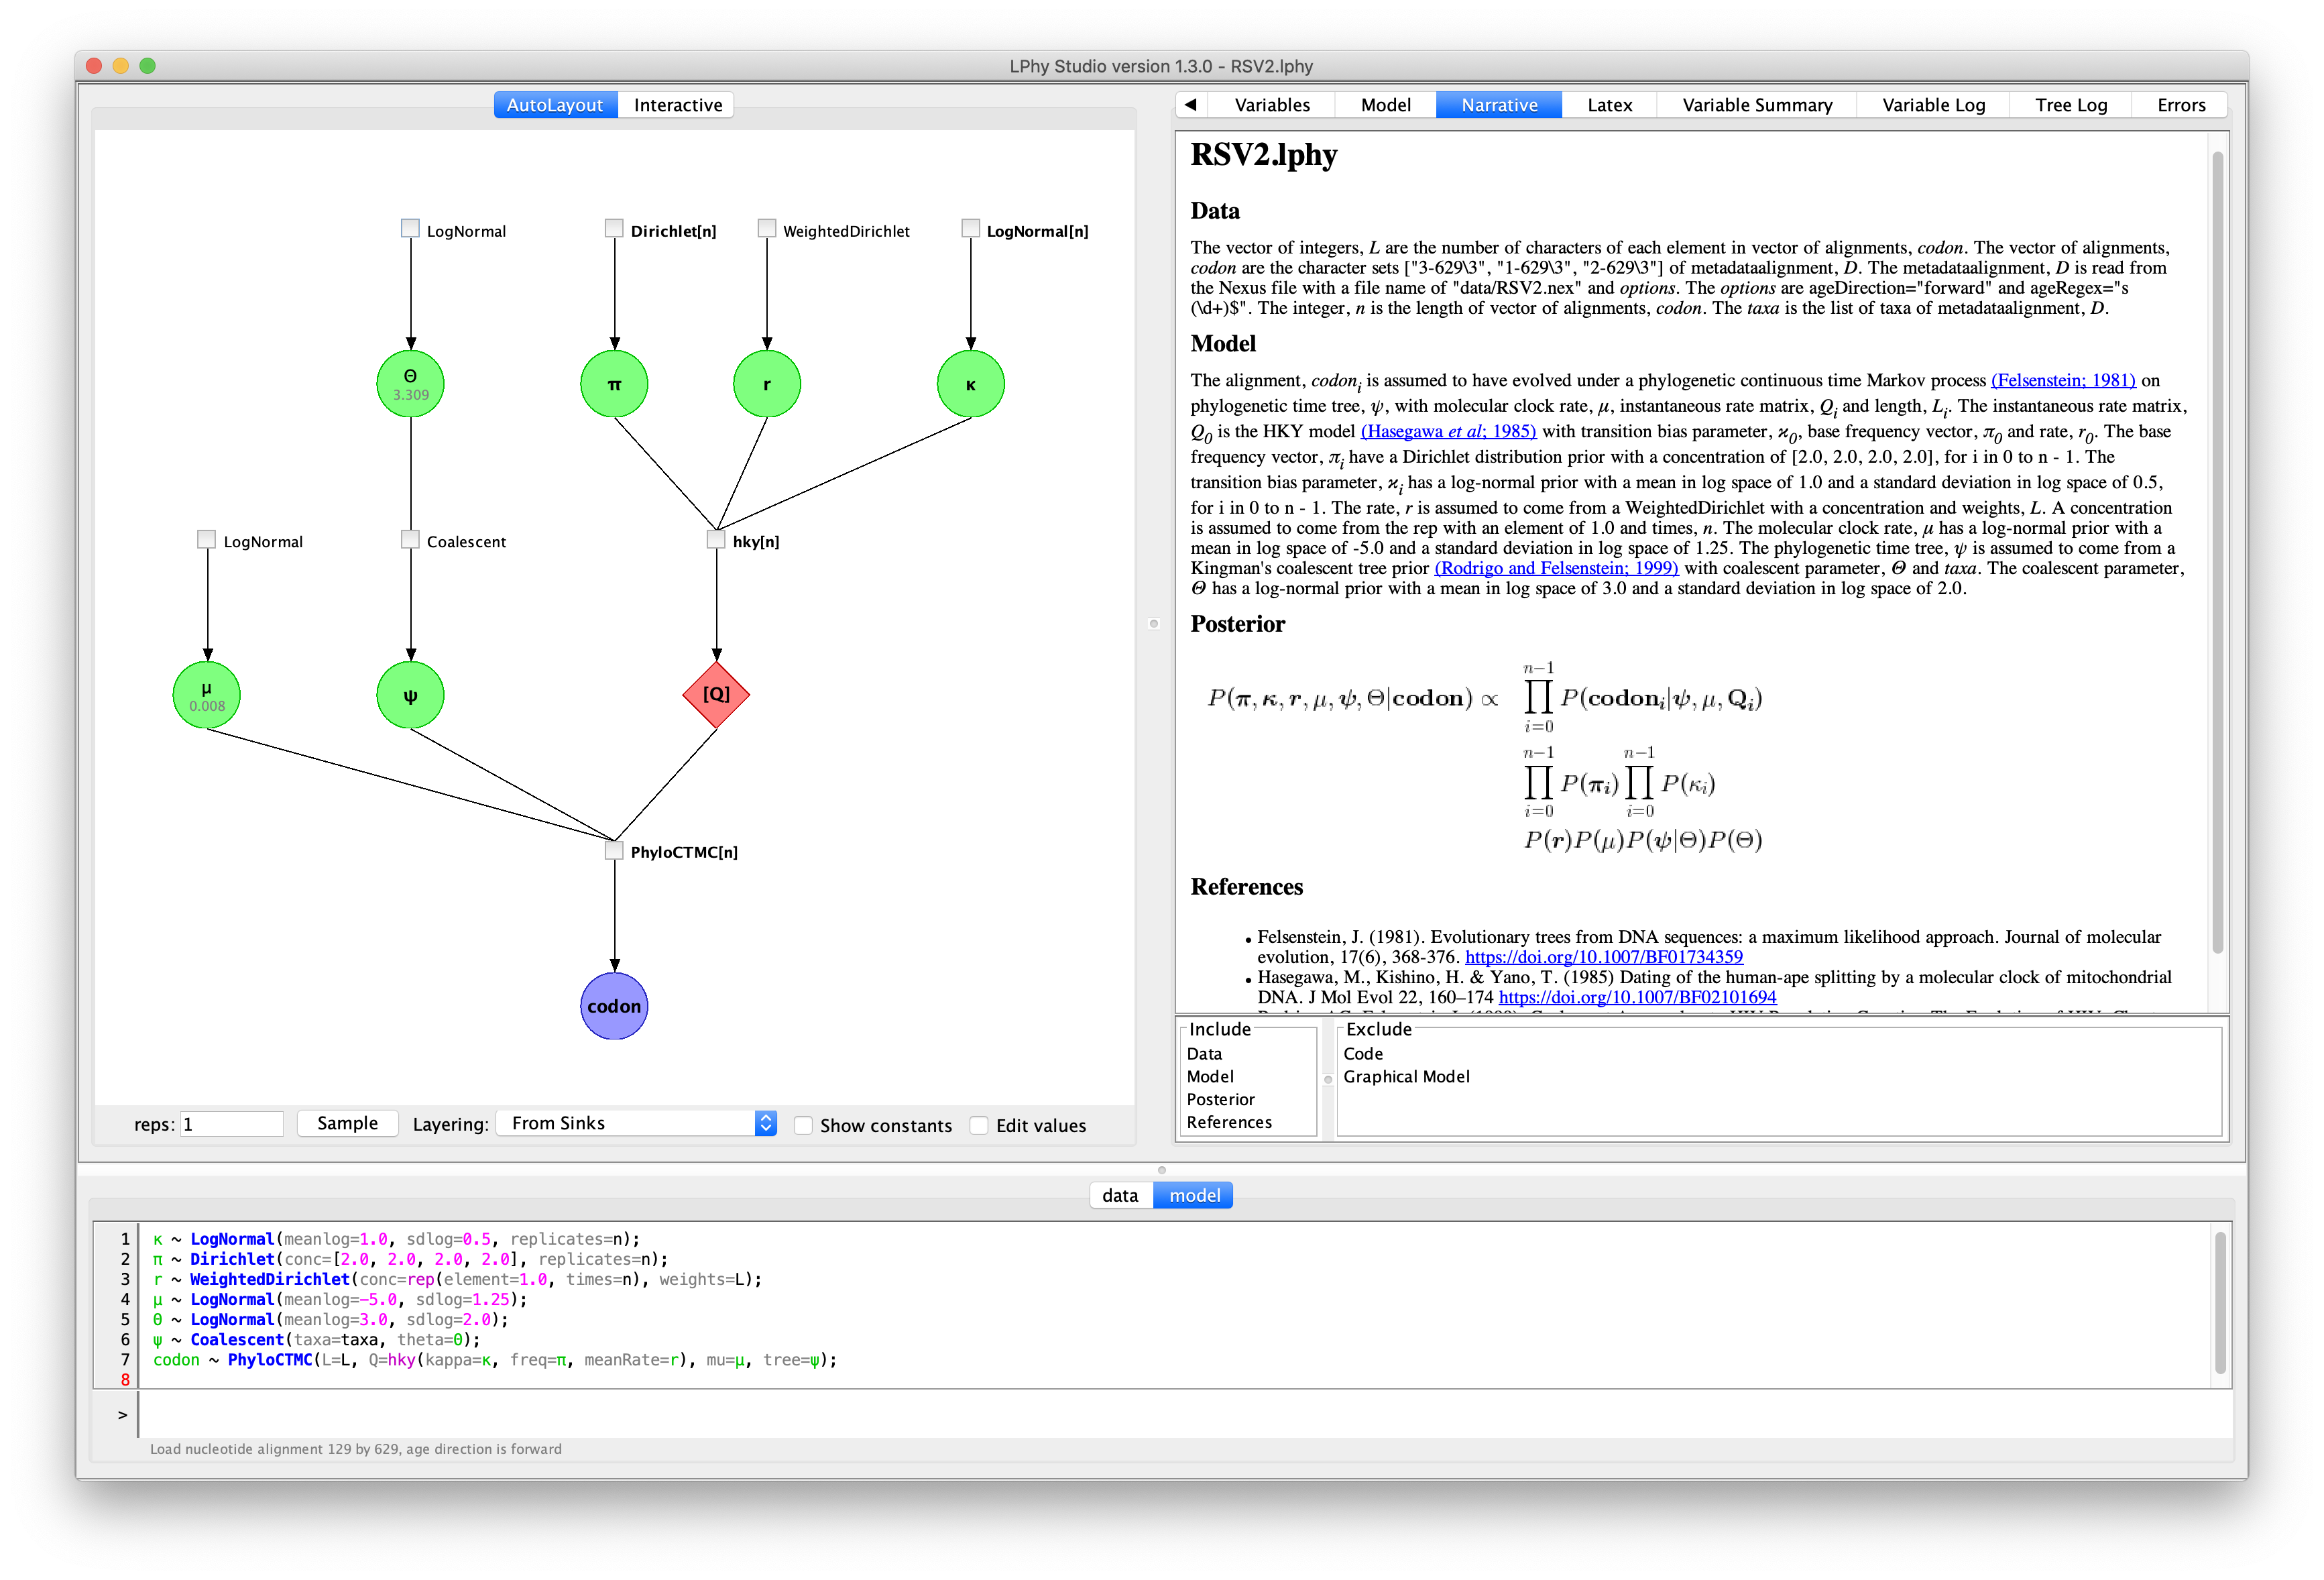
\includegraphics[width=\textwidth]{figs_plos/lphystudio_screenshot.png}
  \caption{A screenshot of LPhy Studio showing the probabilistic graphical model 
  on the left panel (constants hidden), and the auto-generated text description of the data and phylogenetic model on the right panel.} 
  \label{fig:lphystudio}
\end{figure}
Along with the language definition, we introduce LPhy Studio, a GUI intended for (i) model specification, (ii) PGM graphical and textual display, and (iii) simulated data visualization.
Figure \ref{fig:lphystudio} shows a screenshot of LPhyStudio after a simple phylogenetic model was specified. LPhyStudio's additional features include the option to specify models via loading LPhy scripts (rather than building the model line-by-line), and to export PGMs and their descriptions as LaTeX documents.
% \textcolor{red}{\st{The GUI can either import the existing LPhy script or take the script typed from the console on the bottom of LPhy Studio panel. The auto-complete feature is supported when the script is typed in the console. Either way the Studio will guarantee to produce the same graphical probability model representing the specified phylogenetic model. This allows the user focusing on a simple script while sharing the same visualizations across different collaborators.}}

\subsection{LPhy and BEAST2}
\label{sec:lphybeast}
To facilitate the application of specified models for evolutionary inference, the companion program ``LPhyBEAST'' was developed as an interface between LPhy and BEAST2.
LPhyBEAST is a command-line tool that takes as input an LPhy script file specifying a model and clamping data, and produces a BEAST2 XML file as output.

\subsection{A community resource}
LPhy, LPhySTudio and LPhyBEAST were developed to support both end-users and model developers.
As such, this suite of programs is accompanied by extensive documentation and a growing list of tutorials (available on \url{https://linguaphylo.github.io/tutorials/}) covering common use cases and extension mechanisms.
LPhy is designed in a modular fashion: researchers interested in implementing new models within the LPhy language can do so by releasing extension modules that can extend the LPhy application post-deployment.

% \subsection{\textcolor{red}{\st{Extension framework for developers}}}
% \textcolor{\st{The extensibility of a software is extremely important to encourage the future growth and collaborations. 
% LPhy and LPhy extensions are developed based on Java 17 which is the latest long-term support (LTS) version at the time of writing. 
% The LPhy extension mechanism is implemented by using the Java Platform Module System (JPMS) combined with the Service Provider Interface (SPI).}}

% \textcolor{red}{\st{Using this mechanism, the extension developer can develop their own generative distributions and deterministic functions in a separate extension module, and make an individual release.
% The user will easily enjoy these new features, by simply dropping the released jar file into the LPhy library deployment folder.}}

% \textcolor{red}{\st{The LPhy project is a Gradle project from the perspective of developers. Gradle (https://docs.gradle.org) is not only a build system (c.f. ANT), but also contains dependency management, structuring project, and other advanced features. 
% It is well supported by popular IDEs (integrated development environments), such as IntelliJ, so the LPhy core and extension developers can easily share the same software ecosystem and project configurations during development. 
% It integrates with a dependency manager, which helps developers to avoid ``dependency hell".}}

% Another attractive feature of Gradle is that it provides a rich API and many plugins to support the multiple stages of the software build, test, release, and deploying cycle, which helps to define the code conventions and automate the steps of delivering LPhy software and its extensions.  

% \begin{itemize}
% \item for evolutionary biologists
% \begin{enumerate}
% \item describe complex phylogenetic models succinctly and exactly
% \item simulate prior distributions from these models, including arbitrary statistics
% \item use model description to run inference on a real data set using LPhyBEAST
% \item produce precise methods section and graphical model figure for describing analyses in published works
% \end{enumerate}
% \item for computational biologists
% \begin{enumerate}
% \item enable easy extension of the type system and generative distributions available using the extension mechanism of Lingua Phylo Studio (in Java programming language)
% \item implement MCMC inference in BEAST2 for new models using LPhyBEAST and its extension mechanism
% \item do well-calibrated simulation study that validate the implementation of inference framework
% \end{enumerate}
% \end{itemize}

% \newline

\section{Results}
We present key features of the LPhy software using the GT16 substitution and error models \cite{kozlov2022cellphy}. 
Starting from an LPhy script, our software generates a text description of the model, a graphical representation of the model (i.e., a PGM), and multiple displays of the simulated data. 
Additionally, we showcase how LPhy can be used to validate the correctness of the BEAST 2 implementation of GT16 \cite{chen2022accounting}. 

% \subsection{LPhy script}
% An LPhy script consists of a \textbf{data block} which specifies the observed data and a \textbf{model block} which specifies the phylogenetic model. 
% Each block is defined by a set of curly brackets such as in Example \ref{lphy:jccoal}.
% \textcolor{red}{From Walter: can we agree for all code to indent 2 spaces before the data and model block, and 4 spaces (in total) before any commands no matter there is a data / model keyword or not?}
% \textcolor{green}{Show RSV example script or Phylonco script}

% \subsubsection*{LPhyStudio graphical user interface}
\begin{figure}[!ht]
    \centering
    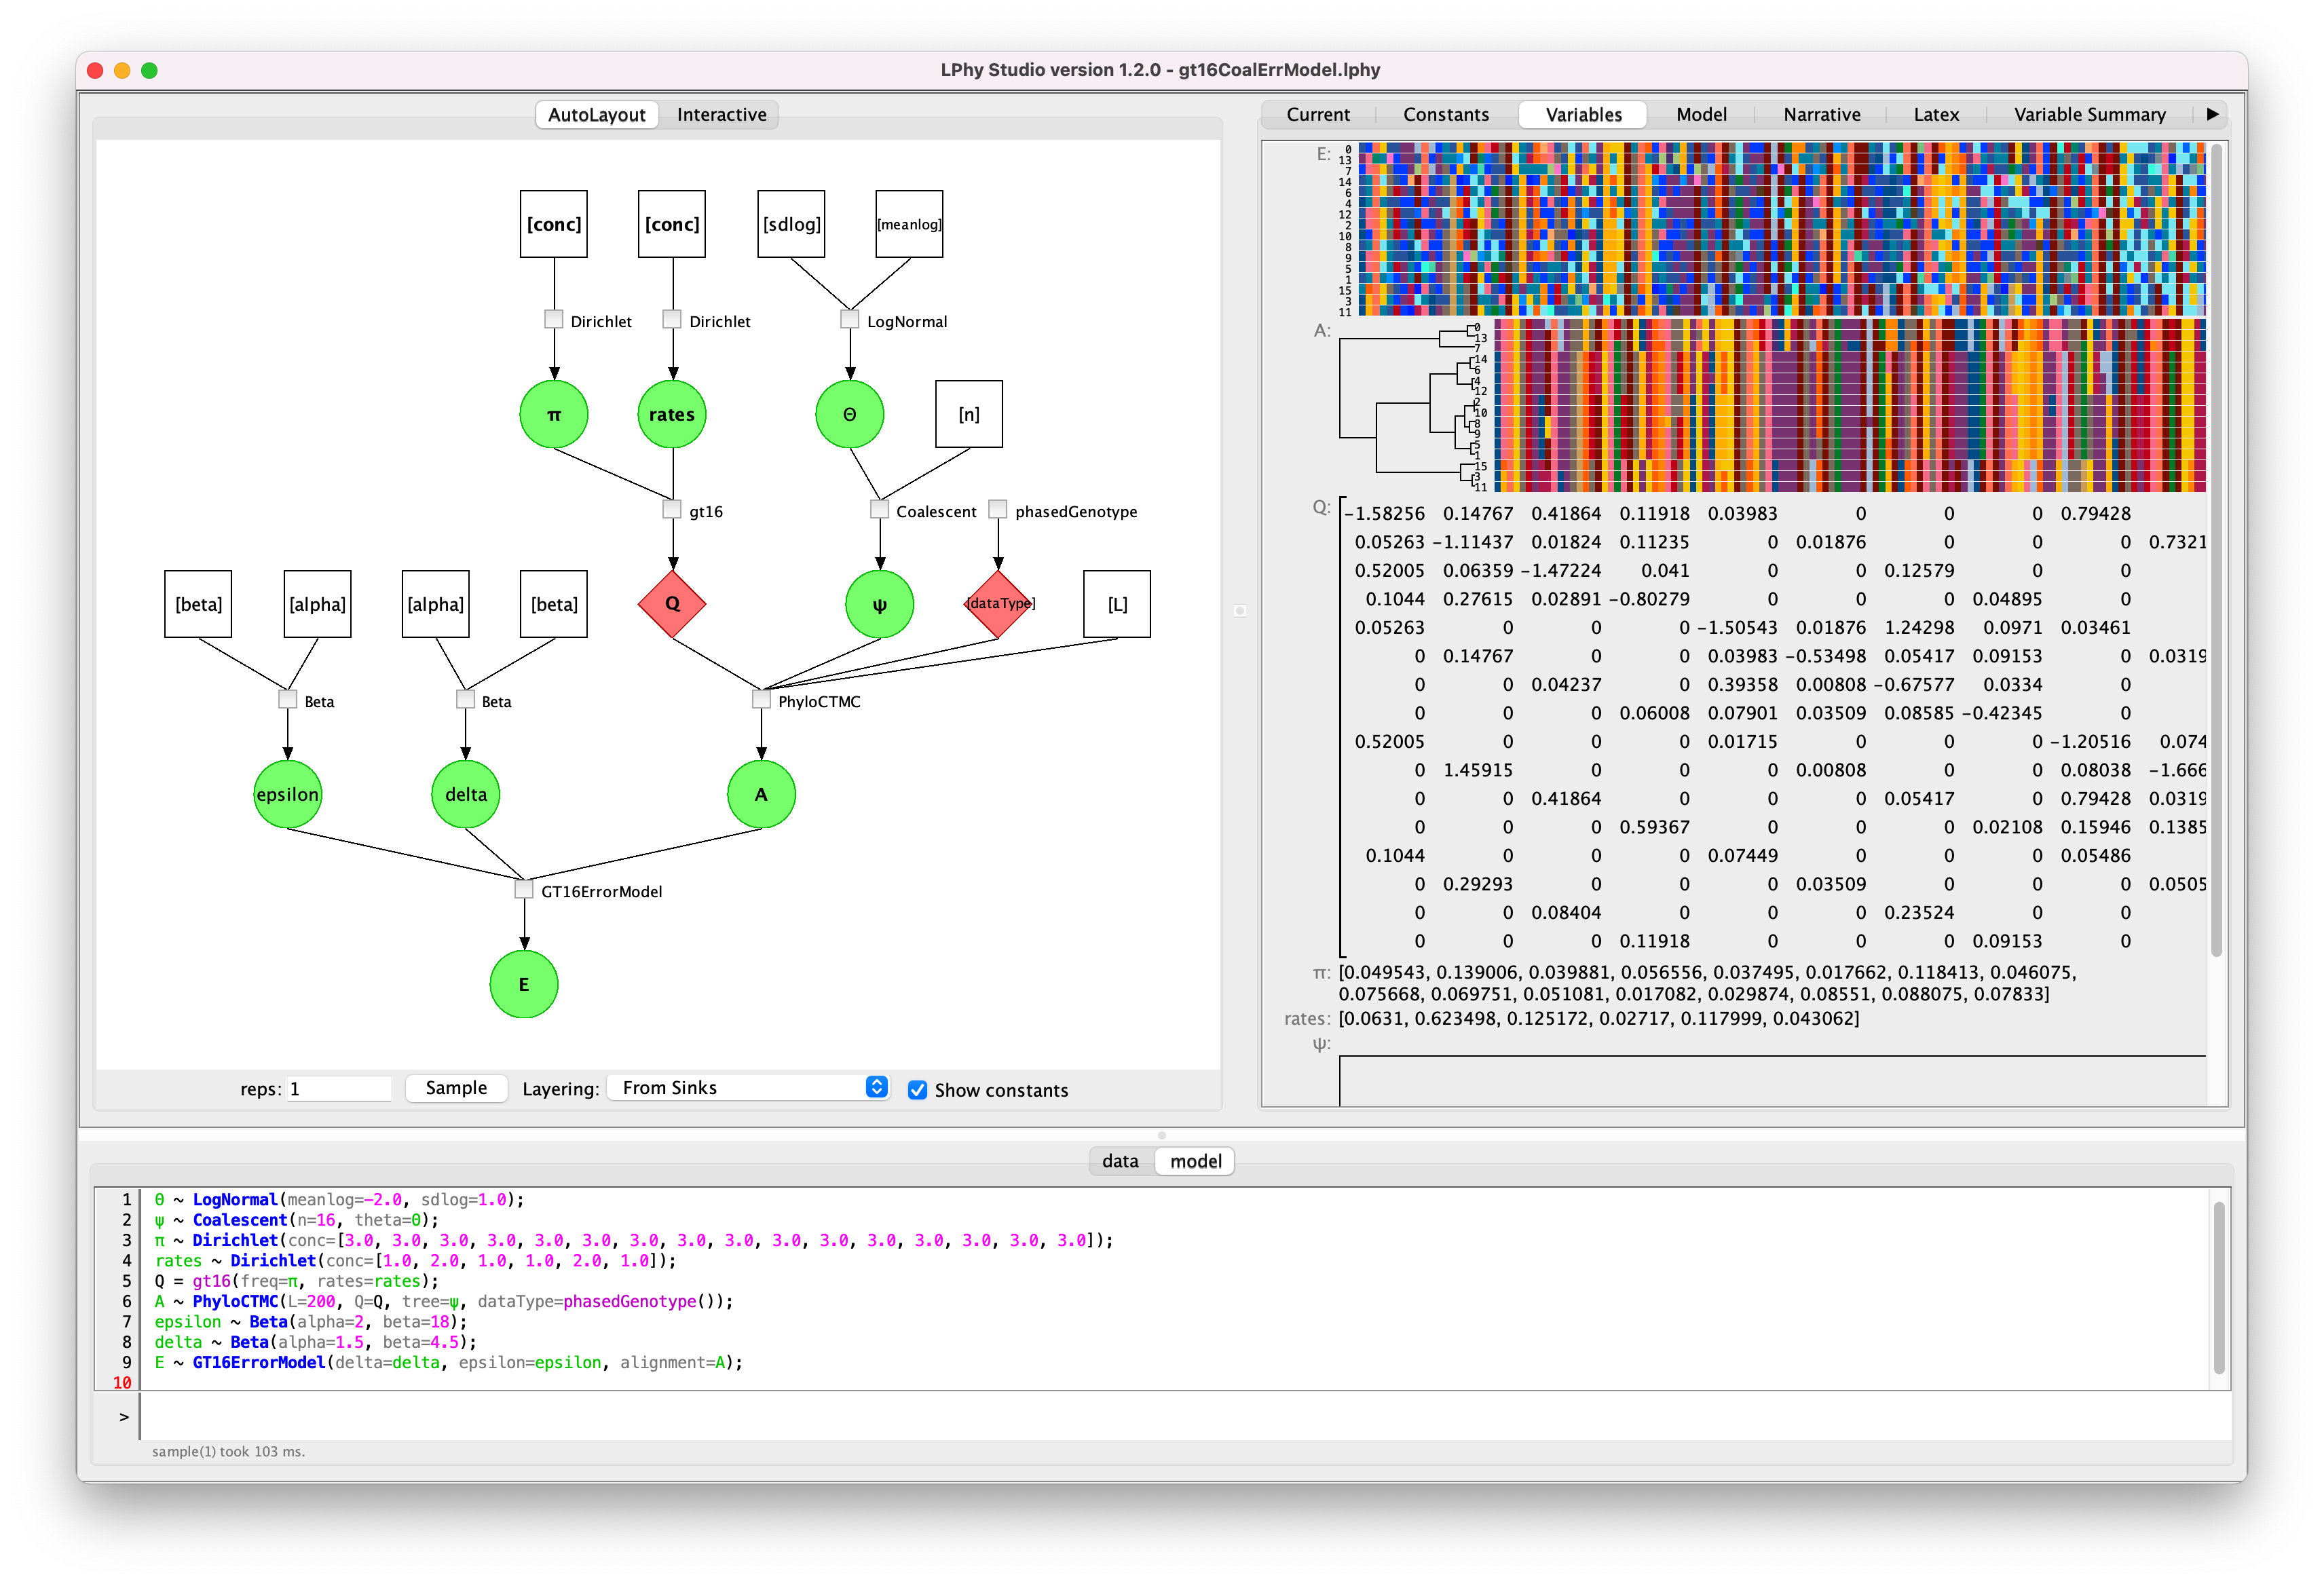
\includegraphics[width=\textwidth]{figs_plos/lphystudio-gt16-mac.jpg}
    \caption{A screenshot of LPhyStudio showing the GT16 substitution and error model \cite{kozlov2022cellphy, chen2022accounting}. 
    The left panel shows the graphical model representation, the right panel shows the simulated tree and diploid nucleotide genotypes, and the bottom panel shows the LPhy script. }
\end{figure}

\subsubsection*{LPhy script}
We start from an LPhy script below which specifies a GT16 substitution and error model \cite{kozlov2022cellphy} for single-cell diploid nucleotides with sequencing and allelic dropout error.

\begin{listing}
\small
\begin{alltt}
model \{
  \textcolor{green}{\(\pi\)}  ~ \textcolor{blue}{Dirichlet}(\textcolor{gray}{conc=}[\textcolor{magenta}{3.0}, \textcolor{magenta}{3.0}, \textcolor{magenta}{3.0}, \textcolor{magenta}{3.0},
  \quad \quad \quad \quad \quad \quad \quad \textcolor{magenta}{3.0}, \textcolor{magenta}{3.0}, \textcolor{magenta}{3.0}, \textcolor{magenta}{3.0}, 
  \quad \quad \quad \quad \quad \quad \quad \textcolor{magenta}{3.0}, \textcolor{magenta}{3.0}, \textcolor{magenta}{3.0}, \textcolor{magenta}{3.0}, 
  \quad \quad \quad \quad \quad \quad \quad \textcolor{magenta}{3.0}, \textcolor{magenta}{3.0}, \textcolor{magenta}{3.0}, \textcolor{magenta}{3.0}]);
  \textcolor{green}{rates} ~ \textcolor{blue}{Dirichlet}(\textcolor{gray}{conc=}[\textcolor{magenta}{1.0}, \textcolor{magenta}{2.0}, \textcolor{magenta}{1.0}, \textcolor{magenta}{1.0}, \textcolor{magenta}{2.0}, \textcolor{magenta}{1.0}]);
  Q = \textcolor{magenta!80!black}{gt16}(\textcolor{gray}{rates=}\textcolor{green}{rates}, \textcolor{gray}{freq=}\textcolor{green}{\(\pi\)});
  \textcolor{green}{\(\Theta\)} ~ \textcolor{blue}{LogNormal}(\textcolor{gray}{meanlog=}\textcolor{magenta}{-2.0}, \textcolor{gray}{sdlog=}\textcolor{magenta}{1.0});
  \textcolor{green}{\(\psi\)} ~ \textcolor{blue}{Coalescent}(\textcolor{gray}{n=}\textcolor{magenta}{16}, \textcolor{gray}{theta=}\textcolor{green}{\(\Theta\)});
  \textcolor{green}{A} ~ \textcolor{blue}{PhyloCTMC}(\textcolor{gray}{L=}\textcolor{magenta}{200}, \textcolor{gray}{Q=}Q, \textcolor{gray}{dataType=}\textcolor{magenta!80!black}{phasedGenotype}(), \textcolor{gray}{tree=}\textcolor{green}{\(\psi\)});
  \textcolor{green}{delta} ~ \textcolor{blue}{Beta}(\textcolor{gray}{alpha=}\textcolor{magenta}{1.5}, \textcolor{gray}{beta=}\textcolor{magenta}{4.5});
  \textcolor{green}{epsilon} ~ \textcolor{blue}{Beta}(\textcolor{gray}{alpha=}\textcolor{magenta}{2}, \textcolor{gray}{beta=}\textcolor{magenta}{18});
  \textcolor{green}{E} ~ \textcolor{blue}{GT16ErrorModel}(\textcolor{gray}{alignment=}\textcolor{green}{A}, \textcolor{gray}{delta=}\textcolor{green}{delta}, \textcolor{gray}{epsilon=}\textcolor{green}{epsilon});
\}
\end{alltt}
\caption{Example of an Lphy script for a GT16 substitution and error model for diploid single-cell nucleotide data.}
\end{listing}

% \begin{listing}
% \small
% \begin{alltt}
%   \textcolor{green}{pi} ~ \textcolor{blue}{Dirichlet}(\textcolor{gray}{conc=}[\textcolor{magenta}{3.0}, \textcolor{magenta}{3.0}, \textcolor{magenta}{3.0}, \textcolor{magenta}{3.0},
%   \quad \quad \quad \quad \quad \quad \quad \textcolor{magenta}{3.0}, \textcolor{magenta}{3.0}, \textcolor{magenta}{3.0}, \textcolor{magenta}{3.0}, 
%   \quad \quad \quad \quad \quad \quad \quad \textcolor{magenta}{3.0}, \textcolor{magenta}{3.0}, \textcolor{magenta}{3.0}, \textcolor{magenta}{3.0}, 
%   \quad \quad \quad \quad \quad \quad \quad \textcolor{magenta}{3.0}, \textcolor{magenta}{3.0}, \textcolor{magenta}{3.0}, \textcolor{magenta}{3.0}]);
%   \textcolor{green}{rates} ~ \textcolor{blue}{Dirichlet}(\textcolor{gray}{conc=}[\textcolor{magenta}{1.0}, \textcolor{magenta}{2.0}, \textcolor{magenta}{1.0}, \textcolor{magenta}{1.0}, \textcolor{magenta}{2.0}, \textcolor{magenta}{1.0}]);
%   Q = \textcolor{magenta!80!black}{gt16}(\textcolor{gray}{rates=}\textcolor{green}{rates}, \textcolor{gray}{freq=}\textcolor{green}{pi});
%   \textcolor{green}{theta} ~ \textcolor{blue}{LogNormal}(\textcolor{gray}{meanlog=}\textcolor{magenta}{-2.0}, \textcolor{gray}{sdlog=}\textcolor{magenta}{1.0});
%   \textcolor{green}{T} ~ \textcolor{blue}{Coalescent}(\textcolor{gray}{n=}\textcolor{magenta}{16}, \textcolor{gray}{theta=}\textcolor{green}{theta});
%   \textcolor{green}{G} ~ \textcolor{blue}{PhyloCTMC}(\textcolor{gray}{L=}\textcolor{magenta}{200}, \textcolor{gray}{Q=}Q, \textcolor{gray}{dataType=}\textcolor{magenta!80!black}{phasedGenotype}(), \textcolor{gray}{tree=}\textcolor{green}{T});
%   \textcolor{green}{delta} ~ \textcolor{blue}{Beta}(\textcolor{gray}{alpha=}\textcolor{magenta}{1.5}, \textcolor{gray}{beta=}\textcolor{magenta}{4.5});
%   \textcolor{green}{epsilon} ~ \textcolor{blue}{Beta}(\textcolor{gray}{alpha=}\textcolor{magenta}{2}, \textcolor{gray}{beta=}\textcolor{magenta}{18});
%   \textcolor{green}{D} ~ \textcolor{blue}{GT16ErrorModel}(\textcolor{gray}{alignment=}\textcolor{green}{G}, \textcolor{gray}{delta=}\textcolor{green}{delta}, \textcolor{gray}{epsilon=}\textcolor{green}{epsilon});
% \end{alltt}
% \caption{Example of an Lphy script for a GT16 substitution and error model for diploid single-cell nucleotide data.}
% \end{listing}


% \begin{figure}[!h]
% \begin{center}
% \begin{scaletikzpicturetowidth}{0.45\textwidth}
% \begin{tikzpicture}[scale=\tikzscale,
% dstyle/.style={draw=blue!50,fill=blue!20},
% vstyle/.style={draw=green,fill=green!20},
% cstyle/.style={font=\small},
% detstyle/.style={draw=red!50,fill=red!20}
% ]
% \node[latent, vstyle] at (0.0, -1.2) (theta) {$\textrm{theta}$};
% \node[latent, vstyle] at (2.4, -1.2) (pi) {$\boldsymbol{\textbf{pi}}$};
% \node[latent, vstyle] at (4.8, -1.2) (rates) {$\boldsymbol{\textbf{rates}}$};
% \node[latent, vstyle] at (0.0, -3.5999999999999996) (T) {$\boldsymbol{T}$};
% \node[det, detstyle] at (3.0, -3.5999999999999996) (Q) {$\boldsymbol{Q}$};
% \node[latent, vstyle] at (1.7999999999999998, -6.0) (G) {$\boldsymbol{G}$};
% \node[latent, vstyle] at (4.2, -6.0) (epsilon) {$\textrm{epsilon}$};
% \node[latent, vstyle] at (6.6, -6.0) (delta) {$\textrm{delta}$};
% \node[latent, vstyle] at (3.5999999999999996, -8.4) (D) {$\boldsymbol{D}$};
% \factor[above=of theta] {LogNormaltheta} {left:\scriptsize LogNormal} {} {} ; %
% \factoredge {} {LogNormaltheta} {theta}; %
% \factor[above=of pi] {Dirichletpi} {left:\scriptsize Dirichlet} {} {} ; %
% \factoredge {} {Dirichletpi} {pi}; %
% \factor[above=of rates] {Dirichletrates} {left:\scriptsize Dirichlet} {} {} ; %
% \factoredge {} {Dirichletrates} {rates}; %
% \factor[above=of T] {CoalescentT} {left:\scriptsize Coalescent} {} {} ; %
% \factoredge {theta} {CoalescentT} {T}; %
% \factor[above=of Q] {gt16Q} {left:\scriptsize gt16} {} {} ; %
% \factoredge {pi, rates} {gt16Q} {Q}; %
% \factor[above=of G] {PhyloCTMCG} {left:\scriptsize PhyloCTMC} {} {} ; %
% \factoredge {Q, T} {PhyloCTMCG} {G}; %
% \factor[above=of epsilon] {Betaepsilon} {left:\scriptsize Beta} {} {} ; %
% \factoredge {} {Betaepsilon} {epsilon}; %
% \factor[above=of delta] {Betadelta} {left:\scriptsize Beta} {} {} ; %
% \factoredge {} {Betadelta} {delta}; %
% \factor[above=of D] {GT16ErrorModelD} {left:\scriptsize GT16ErrorModel} {} {} ; %
% \factoredge {G, delta, epsilon} {GT16ErrorModelD} {D}; %
% \end{tikzpicture}
% \end{scaletikzpicturetowidth}
% \caption{A probabilistic graphical model representation of the GT16 substitution and error model.}
% \end{center}
% \end{figure}

% On the other hand, in the phylogenetic Bayesian inference framework, because of the way we have factorized the joint probability for the data and model parameters, we are implicitly assuming that the alignment could have been produced in a well-known fashion: sampling parameters and tree from their priors, and then simulating the sequence alignment from these sampled parameters and tree. 
%%%neutrality assumption \url{http://alexeidrummond.org/bayesian_phylo_lectures/lecture9} 3rd slide
% This process, known as simulations, can be replicated by following the arrows from the top of the graphical models to the bottom,
% which produces a simulated sequence alignment from the specified phylogenetic model as a result.

% When we follow the arrows backwards, namely from the bottom to the top, we can apply the observed data (sequence alignment) to the model through the phylogenetic Bayesian inference engine, so as to estimate the parameters and tree\cite{hohna2014probabilistic}. 
% The second approach can be done by using data clamping introduced in Section \ref{sec:dataclamping} and combining with a LPhy integration LPhyBEAST introduced in Section \ref{sec:lphybeast}.

% The narrative generator integrated with LPhyStudio can automatically create human-readable descriptions about the data, model, and posterior distribution. 
% It also includes the mathematical definition of the posterior of the given model, and some relevant academic references regarding the model. 
% The generator can also produce these contents in a Latex format, so that the user could simply copy them into a publication manuscript as the reference of the model applied. 
% This will take most researchers in an easy way to precisely describe their models for publishing a Bayesian phylogenetic analysis. 
% \newline
% \newline

\subsubsection*{Natural text description}
\noindent LPhyStudio automatically generates a text description of the model above:
\begin{quote}
The alignment, $\boldsymbol{E}$ is assumed to come from a GT16ErrorModel.
The alignment, $\boldsymbol{A}$ is assumed to have evolved under a phylogenetic continuous time Markov process \cite{felsenstein1981} on  phylogenetic time tree, $\boldsymbol{\psi}$, with  instantaneous rate matrix, $\boldsymbol{Q}$, a length of 200 and a dataType.
The instantaneous rate matrix, $\boldsymbol{Q}$ is the general time-reversible rate matrix on phased genotypes \cite{kozlov2022cellphy} with relative rates, $\boldsymbol{\textbf{rates}}$ and base frequencies, $\boldsymbol{\pi}$.
The base frequencies, $\boldsymbol{\pi}$ have a Dirichlet distribution prior with a concentration of [3.0, 3.0, 3.0, 3.0, 3.0, 3.0, 3.0, 3.0, 3.0, 3.0, 3.0, 3.0, 3.0, 3.0, 3.0, 3.0].
The relative rates, $\boldsymbol{\textbf{rates}}$ have a Dirichlet distribution prior with a concentration of [1.0, 2.0, 1.0, 1.0, 2.0, 1.0].
The dataType is the phased genotype data type.
The phylogenetic time tree, $\boldsymbol{\psi}$ is assumed to come from a Kingman's coalescent tree prior \cite{kingman82} with  coalescent parameter, $\Theta$ and an n of 16.
The coalescent parameter, $\Theta$ has a log-normal prior with a mean in log space of -2.0 and a standard deviation in log space of 1.0.
The $\textrm{delta}$ has a Beta distribution prior with an alpha of 1.5 and a beta of 4.5.
The $\textrm{epsilon}$ has a Beta distribution prior with an alpha of 2 and a beta of 18.
\end{quote}
% \begin{quote}
% The alignment, $\boldsymbol{D}$ is assumed to come from a GT16ErrorModel.
% The alignment, $\boldsymbol{G}$ is assumed to have evolved under a phylogenetic continuous time Markov process \cite{felsenstein1981} on phylogenetic time tree, $\boldsymbol{T}$, with  instantaneous rate matrix, $\boldsymbol{Q}$, a length of 200 and a dataType.
% The instantaneous rate matrix, $\boldsymbol{Q}$ is the general time-reversible rate matrix on phased genotypes \cite{kozlov2022cellphy} with relative rates, $\boldsymbol{\textbf{rates}}$ and base frequencies, $\boldsymbol{\textbf{pi}}$.
% The base frequencies, $\boldsymbol{\textbf{pi}}$ have a Dirichlet distribution prior with a concentration of [3.0, 3.0, 3.0, 3.0, 3.0, 3.0, 3.0, 3.0, 3.0, 3.0, 3.0, 3.0, 3.0, 3.0, 3.0, 3.0].
% The relative rates, $\boldsymbol{\textbf{rates}}$ have a Dirichlet distribution prior with a concentration of [1.0, 2.0, 1.0, 1.0, 2.0, 1.0].
% The dataType is the phased genotype data type.
% The phylogenetic time tree, $\boldsymbol{T}$ is assumed to come from a Kingman's coalescent tree prior \cite{kingman82} with  coalescent parameter, $\textrm{theta}$ and an n of 16.
% The coalescent parameter, $\textrm{theta}$ has a log-normal prior with a mean in log space of -2.0 and a standard deviation in log space of 1.0.
% The $\textrm{delta}$ has a Beta distribution prior with an alpha of 1.5 and a beta of 4.5.
% The $\textrm{epsilon}$ has a Beta distribution prior with an alpha of 2 and a beta of 18.    
% \end{quote}
% \end{tcolorbox}

This natural text narrative can provide a precise starting point for the model description section in a research article.

\subsubsection*{Model validation}
\begin{figure}[!h]
    \centering
    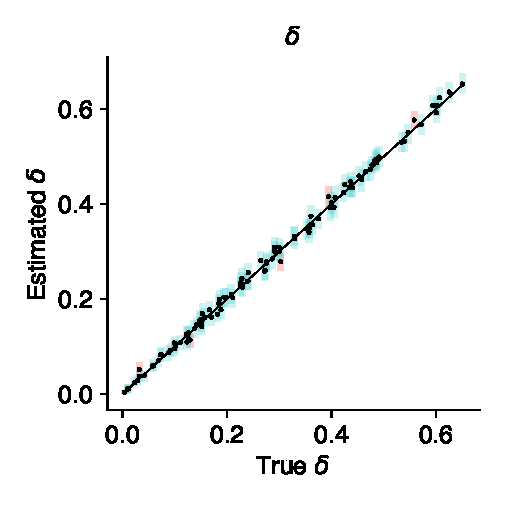
\includegraphics[width=0.25\textwidth]{figs_plos/gt16_EM_delta.pdf}
    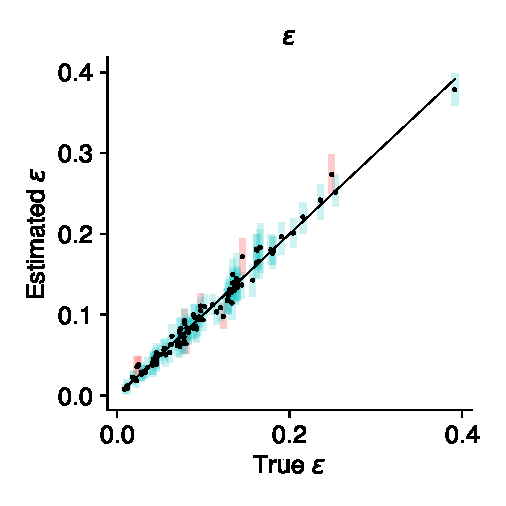
\includegraphics[width=0.25\textwidth]{figs_plos/gt16_EM_epsilon.pdf}
    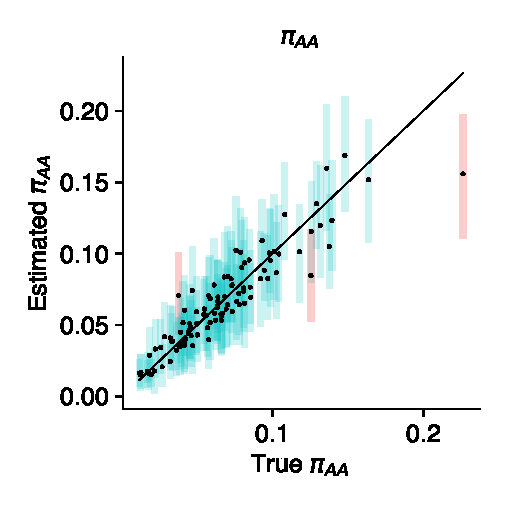
\includegraphics[width=0.25\textwidth]{figs_plos/gt16_EM_pi_0.pdf}
    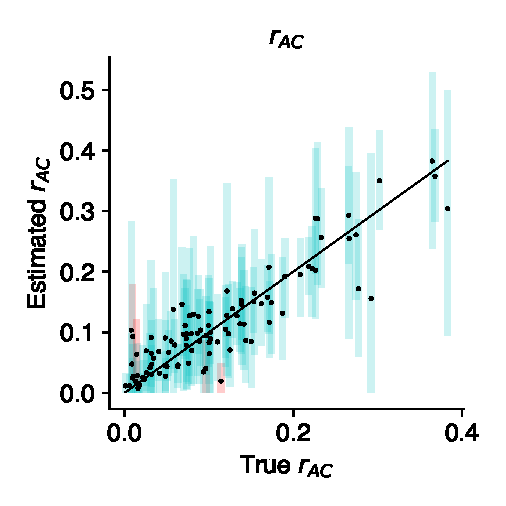
\includegraphics[width=0.25\textwidth]{figs_plos/gt16_EM_rates_ac.pdf}
    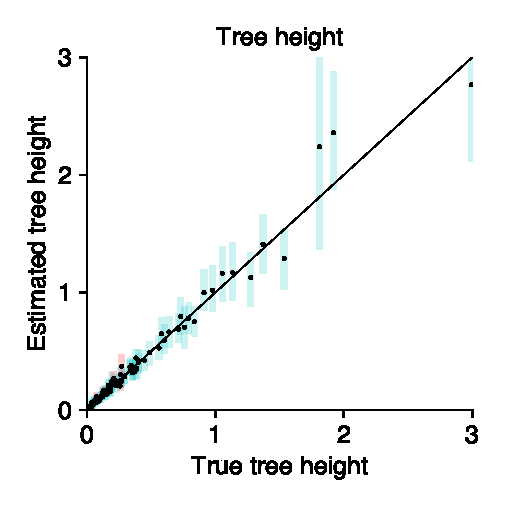
\includegraphics[width=0.25\textwidth]{figs_plos/gt16_EM_treeheight.pdf}
    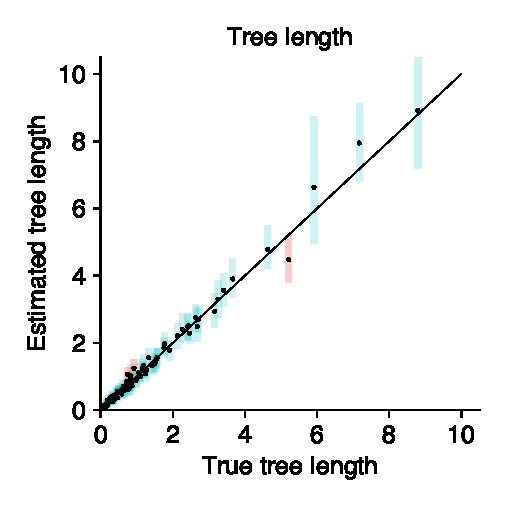
\includegraphics[width=0.25\textwidth]{figs_plos/gt16_EM_treelength.pdf}
    \caption{Model validation for the GT16 diploid nucleotide substitution model and GT16 error model. Each plot shows the 95\% highest posterior density for model parameters: allelic dropout error $\delta$, sequencing error $\epsilon$, equilibrium frequency for $\pi_{AA}$, relative rate $r_{AC}$, tree height, and tree length. }
    \label{fig_validation}
\end{figure}

\noindent The LPhy framework can be used to verify implementation correctness of new models, in which case they are said to be well-calibrated.
Bayesian model validation consists of a series of steps, the first of which is simulation of synthetic data (for recent examples within the BEAST 2 platform, see \cite{gaboriau20,chen2022accounting}). 
By making it possible to simulate under complex models, LPhy greatly simplifies the validation procedure.
Figure \ref{fig_validation} presents the validation results for the model described above, when model specification and simulation were performed using LPhy and LPhyBEAST \cite{chen2022accounting}.

% \subsubsection{Conciser format}
% The code in Example \ref{lphy:jccoal} can be shorten to even 3 lines shown in Example \ref{lphy:jccoal2}, if the constants are not the focus of our study, for instance, simulating alignments from a coalesent model.
% The keywords ``data'', ``model'' and curly brackets are omitted, because the LPhy parser will treat these lines inside the model block as the default.

% {
%   \small
%   \begin{listing}
%     \stepcounter{example}
%     \begin{alltt}
%     \textcolor{green}{\(\Theta\)} ~ \textcolor{blue}{LogNormal}(\textcolor{gray}{meanlog=}\textcolor{magenta}{3.0}, \textcolor{gray}{sdlog=}\textcolor{magenta}{1.0});
%     \textcolor{green}{\(\psi\)} ~ \textcolor{blue}{Coalescent}(\textcolor{gray}{theta=}\textcolor{green}{\(\Theta\)}, \textcolor{gray}{taxa=}\textcolor{magenta!80!black}{taxa}(names=\textcolor{magenta}{1:10}));
%     \textcolor{green}{D} ~ \textcolor{blue}{PhyloCTMC}(\textcolor{gray}{L=}\textcolor{magenta}{200}, \textcolor{gray}{Q=}\textcolor{magenta!80!black}{jukesCantor}(), \textcolor{gray}{tree=}\textcolor{green}{\(\psi\)});
%     \end{alltt}
%     \caption{A 3-line code for Example \ref{lphy:jccoal}.}
%     \label{lphy:jccoal2}
%   \end{listing}
% }

% \subsubsection{Achieving readability, re-usability and reproducibility}
% \textcolor{blue}{TODO: review} All variables and generators in LPhy are named by well-known terms, as well as the parameters. For example, the blue key word ``Coalescent'' in Example \ref{lphy:jccoal} represents a generative distribution to implement Kingman's coalescent tree prior. 
% The variable name in LPhy can be any greek letters, some of which are commonly used to indicate certain parameters in the phylogenetic models. For example, $\Theta$ usually represents the effective population size in a constant-size coalescent model. 

% A LPhy script, such as Example \ref{lphy:jccoal}, can be visualised by a probabilistic graphical model, such as Figure \ref{fig:jccoalPGM}. The variables and generators will be one-to-one mapped to the components of the graphical model, vice versa. 
% Priors are the important part of the specification of a Bayesian phylogenetic model. But this part is often ignored or incompletely described in some publications. The probabilistic graphical model representation naturally solves this issue once the complete graph is delivered.
% It is also very convenient to reuse the same model for a different data (e.g. alignment) or constants by simply replacing the line in the data block.  

% This concise and precise representation of LPhy language is the key driver to improve the reproducibility for Bayesian phylogenetics. The convenience to specify a phylogenetic model using LPhy will greatly encourage the researchers to apply the same methodology in this field.


% % move to supplementary
% \subsubsection{Model averaging using bModelTest}
% It has been a problematic approach to select one ``best-fit'' nucleotide substitution model as well as site model in a deterministic manner while doing a Bayesian phylogenetic analysis. Here the site model is a composited model taking a substitution model as an input, and including the parameters to model the base frequencies, rate heterogeneity across sites, and proportion of invariable sites.

% BModel test \cite{bouckaert2017bmodeltestcomparison} provides model averaging of substitution models and site models. 
% If the substitution and site model are not of direct interest, then bModelTest provides estimates of the phylogeny averaged over substitution models and site models; otherwise, if they are of interest, then bModelTest provides a posterior distribution over these models. \cite{bouckaert2019beastanalysis}

% {\small
%   \begin{alltt}
%     \textcolor{green}{\(\pi\)} ~ \textcolor{blue}{Dirichlet}(\textcolor{gray}{conc=}[\textcolor{magenta}{3.0}, \textcolor{magenta}{3.0}, \textcolor{magenta}{3.0}, \textcolor{magenta}{3.0}]);
%     \textcolor{green}{rates} ~ \textcolor{blue}{Dirichlet}(\textcolor{gray}{conc=}[\textcolor{magenta}{1.0}, \textcolor{magenta}{2.0}, \textcolor{magenta}{1.0}, \textcolor{magenta}{1.0}, \textcolor{magenta}{2.0}, \textcolor{magenta}{1.0}]);
%     \textcolor{black}{modelSet = }\textcolor{magenta!80!black}{bModelSet}(\textcolor{magenta}{"transitionTransversionSplit"});
%     \textcolor{green}{M} ~ \textcolor{blue}{DiscreteUniform}(\textcolor{gray}{lower=}\textcolor{magenta}{0}, \textcolor{gray}{upper=}modelSet.\textcolor{magenta}{size}()-\textcolor{magenta}{1});
%     \textcolor{black}{Q = }\textcolor{magenta!80!black}{nucleotideModel}(\textcolor{gray}{modelSet=}\textcolor{green}{modelSet}, \textcolor{gray}{modelIndicator=}\textcolor{green}{M}, \textcolor{gray}{freq=}\textcolor{green}{\(\pi\)}, \textcolor{gray}{rates=}\textcolor{green}{rates});
% \end{alltt}
% }

% The above lines are the first part of code to specify a bModelTest analysis using LPhy, 
% where $\pi$ is an array of the nucleotide base frequencies and the $rates$ variable contains the relative rates of the GTR process. They are separately sampled from two different Dirichlet distributions.  
% The third line declares the model space is restricted to the set of substitution models that allow grouping only within transitions and within transversions\cite{bouckaert2019beastanalysis}, where the deterministic variable $modelSet$ encapsulates an instance instantiated from the object BModelSet for this information.
% The index of the substitution model to be employed $M$ will be sampled uniformly from a range of 0 and the size of the returned model set minus one.
% Here the code $modelSet.size()$ is called as ``method call'' in LPhy, which is a method that is similar to a LPhy function but has to be called from an object. 
% The instantaneous rate matrix $Q$ is then determined by given these parameters.
  
% {\small
%   \begin{alltt}  
%     \textcolor{green}{siteRates} ~ \textcolor{blue}{DiscretizeGamma}(\textcolor{gray}{alpha=}\textcolor{magenta}{0.5}, \textcolor{gray}{ncat=}\textcolor{magenta}{4}, \textcolor{gray}{replicates=}\textcolor{magenta}{200});
%     \textcolor{green}{pInv} ~ \textcolor{blue}{Beta}(\textcolor{gray}{alpha=}\textcolor{magenta}{1.0},\textcolor{gray}{beta=}\textcolor{magenta}{1.0});
%     \textcolor{green}{I_siteRates} ~ \textcolor{blue}{Bernoulli}(\textcolor{gray}{p=}\textcolor{magenta}{0.5});
%     \textcolor{green}{I_pInv} ~ \textcolor{blue}{Bernoulli}(\textcolor{gray}{p=}\textcolor{magenta}{0.5});
%     \textcolor{black}{siteModel = }\textcolor{magenta!80!black}{bSiteModel}(\textcolor{gray}{Q=}\textcolor{green}{Q}, \textcolor{gray}{siteRates=}\textcolor{green}{siteRates}, \textcolor{gray}{pInv=}\textcolor{green}{pInv}, \\ \textcolor{gray}{useSiteRates=}\textcolor{green}{I_siteRates}, \textcolor{gray}{usePInv=}\textcolor{green}{I_pInv}); 
%   \end{alltt}
% }

% The second part of code specifies model averaging of site models.
% The 200 raw site rates are drawn from a DiscretizeGamma with a shape of 0.5 and a ncat of 4 and store into the variable $siteRates$.
% The proportion of invariable sites $pInv$ has a Beta distribution prior with an alpha of 1.0 and a beta of 1.0. 
% The site rate heterogeneity indicator $I\_siteRates$ will be true if the site rates have heterogeneity.
% The proportion invariable indicator $I\_pInv$ will be true if the proportion invariable used.
% Both has a coin toss distribution prior. 

% The last line below shows how it is used in PhyloCTMC.

% {\small
%   \begin{alltt}  
%     \textcolor{green}{D} ~ \textcolor{blue}{PhyloCTMC}(\textcolor{gray}{L=}\textcolor{magenta}{200}, \textcolor{gray}{siteModel=}siteModel, \textcolor{gray}{tree=}\textcolor{green}{\(\psi\)});
%   \end{alltt}
% }

 


% \subsection*{Tree generative distributions}

% There are many statistical programming languages such as Stan
% \cite{carpenter2017stan}, JAGS \cite{plummer2003jags} and BUGS \cite{lunn2009bugs, gilks1994language} that provide the possibility
% of succinctly describing statistical models. The unique model feature of
% phylogenetic analysis is the phylogenetic tree.
% This is a complex high-dimensional object, part discrete, part
% continuous.
% There is no bijection between tree space and Euclidean space, so it
% can not be treated with standard statistical distributions.
% As a result specialist software is needed to perform inference \cite{hohna2016revbayes,bouckaert2019beastanalysis}.

% The aim of LPhy is describe the standard phylogenetic tree
% distributions succinctly and precisely, while leaving out trivial algorithmic details related to the method
% of inference and the particular software employed to do the inference.

% \subsubsection*{Coalescent generative distributions for time trees}

% LPhy has describes a family of coalescent generative distributions
% that produce TimeTrees.

% The simplest model in this package is the one parameter model
% constant-population size coalescent.
% The generation-time-scaled population size parameter (theta) parameter determines at
% what rate, per unit time, a pair of lineages coalesce, backwards in time.

% \subsubsection*{Constant population size coalescent model}

% In its simplest form \cite{kingman81} the coalescent model produces a
% tree on a fixed number of leaves based on a population size parameter (theta):

% \begin{alltt}
%   g ~ Coalescent(theta=0.1, n=16);
% \end{alltt}

% It is also possible to give explicit taxa labels to the generative
% distribution:

% \begin{alltt}
%   g ~ Coalescent(theta=0.1, taxa=["a", "b", "c", "d"]);
% \end{alltt}

% It is also possible to handle serially-sampled (time-stamped) data by
% adding ages.
% There are two ways to do that:

% Ages without taxa names:

% \begin{alltt}
%   g ~ Coalescent(theta=0.1, ages=[0.0, 0.1, 0.2, 0.3]);
% \end{alltt}

% Ages and taxa names:

% \begin{alltt}
%   taxaAges = taxaAges(taxa=["a", "b", "c", "d"], ages=[0.0, 0.1, 0.2, 0.3]);
%   g ~ Coalescent(theta=0.1, taxaAges=taxaAges);
% \end{alltt}

% \subsubsection*{Classic skyline coalescent model}

% A highly parametric version of the coalescent is also possible, where
% a series of theta values are provided, one for each group of consecutive coalescent intervals.
% If the groupSizes are specified then each coalescent interval is given its
% own population size.
% The following code would generate a tree of five taxa, since there are four theta values provided:

% \begin{alltt}
%   g ~ SkylineCoalescent(theta=[0.1, 0.2, 0.3, 0.4]);
% \end{alltt}

% The theta values are indexed from the present into the past.
% So the first coalescent interval (starting from the leaves)
% would be generated assuming a population size parameter of 0.1, while
% the last coalescent interval (culimating at the root of the tree)
% would be generated from a population size parameter of 0.4.

% It is also possible to add taxa and/or taxa age information:

% \begin{alltt}
%   taxaAges = taxaAges(taxa=["a", "b", "c", "d"], ages=[0.0, 0.1, 0.2, 0.3]);
%   g ~ SkylineCoalescent(theta=[0.1, 0.2, 0.3], taxaAges=taxaAges);
% \end{alltt}

% This will produce a serial coalescent tree with three distinct epochs
% of population size on four taxa with distinct ages.

% \subsubsection*{Generalized skyline coalescent model}

% The following generative distribution call will produce a tree of size
% n=11 taxa, since 4+3+2+1=10= coalescent intervals.
% The first four intervals will all have theta=0.1, the next three will
% have theta=0.2, the next two will have theta=0.3, and the last
% coalescent interval will have theta=0.4:

% \begin{alltt}
%   g ~ SkylineCoalescent(theta=[0.1, 0.2, 0.3, 0.4], groupSizes=[4,3,2,1]);
% \end{alltt}

% \subsubsection*{Structured coalescent}

% A structured coalescent process takes a migration matrix (M) with
% population sizes of each deme on the diagonal:
% For K demes, theta is an K-tuple and the dimension of m is $K^2 -
% K$. $n$ is a tuple of sample sizes, one dimension for each deme:

% \begin{alltt}
%   M = migrationMatrix(theta=[0.1, 0.1], m=[1.0, 1.0]);
%   g ~ StructuredCoalescent(M=M, n=[15, 15]);
% \end{alltt}

% \subsubsection*{Multispecies coalescent}

% This model allows for gene tree-species tree discordance, and is a
% hierarchical model of phylogeny.
% A simple multispecies coalescent model has one distribution define a
% species tree, and a second distribution define a gene tree based on
% the species tree:

% \begin{alltt}
%   S ~ Yule(lambda=5, n=4);
%   theta = [0.1, 0.1, 0.1, 0.1, 0.1, 0.1, 0.1];
%   g ~ MultispeciesCoalescent(theta=theta, n=[2, 2, 2, 2], S=S);
% \end{alltt}

% Each branch in the species tree has its own theta value.
% The $n$ value describes how many individuals are represented in
% the gene tree for each species.
% It is a tuple of integers with length equal to the number of species
% in the species tree.

% \subsubsection*{Birth-death process generative distributions of trees}

% The other main family of tree distributions is the birth-death-sampling generative distributions.

% The simplest model in this family is the one parameter model Yule model \cite{yule1925ii}.
% The birth rate (lambda) parameter determines at what rate, per unit time, each lineage bifurcates to produce two daughter lineages.
% This describes a pure birth process, so that the number of lineages grows monotonically forward in time.

% \subsubsection*{Yule model}

% In its simplest form the Yule model has a stopping criterion based on the final number of leaves in the tree.
% The following code will generate a random Yule tree with 16 leaves:

% \begin{alltt}
%   tree ~ Yule(lambda=1.0, n=16);
% \end{alltt}

% It is also possible to give explicit taxa labels to the generative distribution:

% \begin{alltt}
%   taxa = 1:16;
%   tree ~ Yule(lambda=1.0, taxa=taxa);
% \end{alltt}

% or

% \begin{alltt}
%   taxa = ["A", "B", "C", "D"];
%   tree ~ Yule(lambda=1.0, taxa=taxa);
% \end{alltt}

% \subsubsection*{Calibrated Yule model}

% It is also possible the generate a Yule tree with a given rootAge:

% \begin{alltt}
%   tree ~ Yule(lambda=1.0, n=16, rootAge=10);
% \end{alltt}

% This is useful if you want to produce a calibrated analysis where there is a separate prior on the root age of the tree:

% \begin{alltt}
%   rootAge ~ LogNormal(meanlog=2.0, sdlog=1.0);
%   tree ~ Yule(lambda=1.0, n=16, rootAge=rootAge);
% \end{alltt}

% \subsubsection*{Birth-death model}

% The birth-death tree process is a generalisation of the Yule model. A second rate of extinction (mu) is added alongside
% the rate of speciation (lambda). Running forward in time it is possible for the number of lineages to both grow and
% shrink, and indeed for the tree process to go completely extinct.

% \subsubsection*{Calibrated Birth-Death process}

% A calibrated birth-death process can be describe like so:

% \begin{alltt}
%   tree ~ BirthDeath(lambda=2.0, mu=1.0, n=16, rootAge=10);
% \end{alltt}

% It is important to realise that the resulting tree will contain only the extant lineages. All extinct lineages will be
% suppressed. As with the Yule model it is possible to directly specify the taxa names:

% \begin{alltt}
%   taxa = ["A", "B", "C", "D"];
%   tree ~ BirthDeath(lambda=2.0, mu=1.0, taxa=taxa, rootAge=10);
% \end{alltt}

% \subsubsection*{Full birth-death process}

% It is possible to generate a full birth-death tree that includes also extinct lineages using the following generative
% distribution:

% \begin{alltt}
%   tree ~ FullBirthDeath(lambda=2.0, mu=1.0, rootAge=10);
% \end{alltt}

% Note that unlike the BirthDeath generative distribution, this process will generate a tree with a random number of
% leaf nodes, both in terms of extinct and extant lineages. The only conditioning is on the root age.

% \subsubsection*{Birth-death-sampling process}

% A birth-death-sampling process adds a third parameter (rho) the probability of sampling each extant lineage. Again,
% only extant lineages are leaves in the resulting tree and extinct lineages are suppressed:

% \begin{alltt}
%   T ~ BirthDeathSampling(lambda=2.0, mu=1.0, rho=0.5, rootAge=3);
% \end{alltt}

% An alternative parameterization allows specification of the diversification and turnover rates:

% \begin{alltt}
%   T ~ BirthDeathSampling(diversification=1.0, turnover=0.5, rho=0.5, rootAge=3);
% \end{alltt}

% Again it is important to note that the number of tips of the tree is a random variable, and is not conditioned on,
% unlike for the BirthDeath generative distribution above.

% \subsubsection*{Birth-death-serial-sampling process}

% A birth-death-serial-sampling \cite{stadler2013dating} process adds a fourth parameter (psi), the rate of sampling each lineage per unit time.
% Now leaves of the tree can either be extinct (psi-sampled) or extant (rho-sampled).

% \begin{alltt}
%   ages = [0.0,1.0,2.0,3.0,4.0];
%   tree ~ BirthDeathSerialSampling(lambda=1, mu=0.5, rho=0.1, psi=1, rootAge=5, ages=ages);
% \end{alltt}

% In this case the number of leaves in the tree, and their ages are conditioned on, so are not random variables.


% \subsection*{Models of evolutionary rates and sequence evolution}

% Another key distribution necessary to perform phylogenetic inference
% is the phylogenetic continuous-time Markov process and its inference
% equivalent the phylogenetic likelihood \cite{felsenstein1981}.

% In its simplest form the PhyloCTMC generative
% distribution takes an instantaneous transition matrix (Q), a number of sites (L) and a tree:

% \begin{alltt}
%   tree = newick(tree="((A:0.1,B:0.1):0.2,(C:0.15,D:0.15):0.15);");
%   D ~ PhyloCTMC(tree=tree, Q=jukesCantor(), L=100);
% \end{alltt}

% \subsection*{Molecular clock}

% If the tree is not in units of substitutions per site, then it is possible to include a molecular clock rate
% to scale the branches of the tree from time to substitutions per site. This example will give the same
% result as the previous example, but the tree is now in units of time, so the mutation rate (mu) in units of
% substitutions per site per unit time is given.

% \begin{alltt}
%   tree = newick(tree="((A:10,B:10):20,(C:15,D:15):15);");
%   D ~ PhyloCTMC(tree=tree, Q=jukesCantor(), L=100, mu=0.01);
% \end{alltt}

% \subsection*{ Nucleotide substitution models}

% There are a number of built in functions to construct standard nucleotide rate matrices. Some examples:

% \begin{alltt}
%   jc = jukesCantor();
%   hky = hky(kappa=2.0, freq=[0.2, 0.25, 0.3, 0.25]);
%   gtr = gtr(rates=[0.1, 0.25, 0.15, 0.15, 0.25, 0.1], freq=[0.2, 0.25, 0.3, 0.25]);
% \end{alltt}

% The Dirichlet prior is a natural prior for relative rates and frequencies, so a full model for GTR could
% look like this:

% \begin{alltt}
%   pi ~ Dirichlet(conc=[3.0,3.0,3.0,3.0]); // dirichlet prior on base frequencies
%   R ~ Dirichlet(conc=[1.0, 2.0, 1.0, 1.0, 2.0, 1.0]); // dirichlet prior on relative rates
%   Q = gtr(freq=pi, rates=R); // construct the GTR instantaneous rate matrix
% \end{alltt}

% \subsection*{ Rate heterogeneity across sites}

% The PhyloCTMC generative distribution takes a parameter siteRates to describe rates across sites.
% For inference, a common model is the discretized Gamma distribution of site rate heterogeneity (Yang, 1994).

% To match this model for simulation in LPHY do the following:

% \begin{alltt}
%   tree = newick(tree="((A:0.1,B:0.1):0.2,(C:0.15,D:0.15):0.15);");
%   siteRates ~ G(shape=0.5, ncat=4, reps=100); // generate 100 site rates from a discretized Gamma
%   D ~ PhyloCTMC(tree=tree, Q=jukesCantor(), siteRates=siteRates);
% \end{alltt}

% \subsection*{  Relaxed clock models (rate heterogeneity across branches) }

% The PhyloCTMC generative distribution can also take an optional parameter branchRates to describe the
% rates across branches:

% \begin{alltt}
%   tree = newick(tree="((A:0.1,B:0.1):0.2,(C:0.15,D:0.15):0.15);");
%   branchRates = [0.5, 2.0, 1.0, 1.0, 2.0, 0.5];
%   D ~ PhyloCTMC(L=100, Q=jukesCantor(), tree=tree, branchRates=branchRates);
% \end{alltt}


% Move to supplementary
% \subsection{A model guide for users}
% There are two learning curves for a beginner level of users, one is to learn the LPhy language, the other is to understand the model. To shorten these learning curves, a tool with GUI, called Model Guide, is implemented to list all available LPhy generative distributions and functions in runtime. 
% They are classified into several categories for users to look up easily.

% Selecting a model or function, e.g. Figure \ref{fig:modelguide}, the user can find its usage, description, and the example scripts (they are accessible from LPhy Studio). For a published model, the citation is also provided for the convenience of learning, if it has DOI or book ISBN number, the hyperlink will lead the reader to the online publication.   

% \textcolor{blue}{TODO: Figure to suppl?}

% \begin{figure}
%   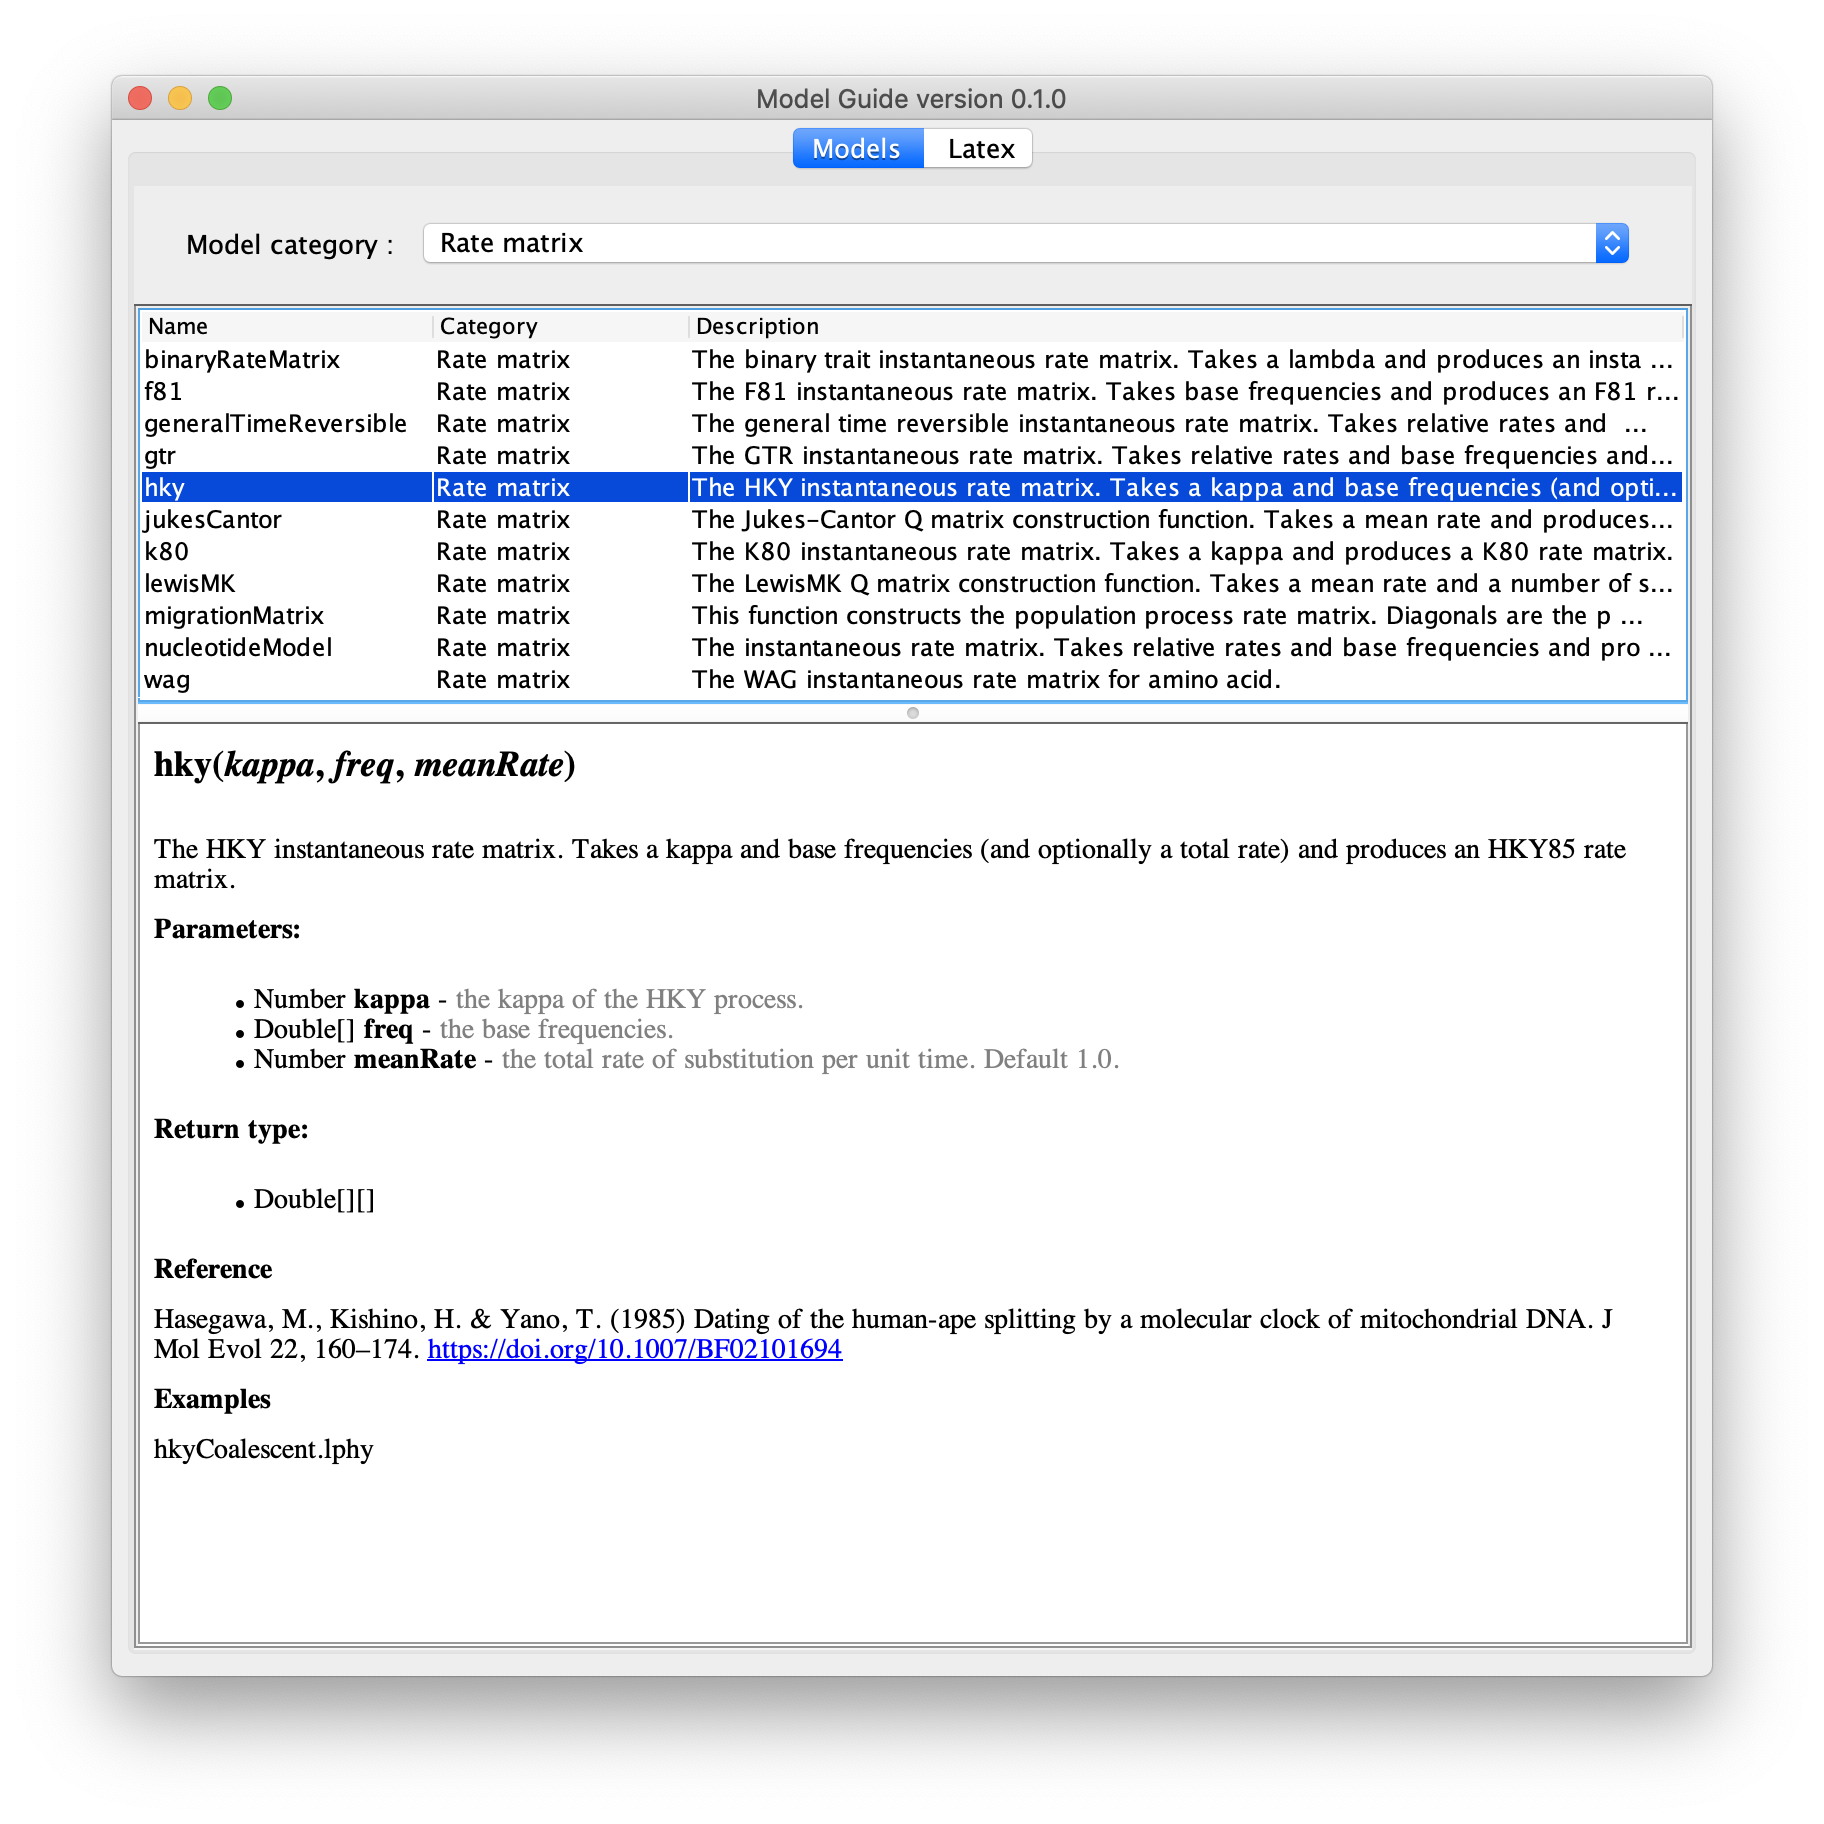
\includegraphics[width=\textwidth]{figs/modelguide.png}
%   \caption{A screenshot of Model Guide showing the usage of \emph{hky} function, its example script, and the citation of HKY85 model.} 
%   \label{fig:modelguide}
% \end{figure}


% \subsection{Data simulations from a phylogenetic model}
% Simulating alignments from a specified model can ever be easy using the LPhy Studio. This can be simply done by loading a LPhy script and then clicking the ``Sample" button. 
% It logs both ``true" values of the parameters and ``true" trees simulated from the specified model defined in the LPhy script. 
% The result of running 100 simulations from the simple HKY+Coalescent model is illustrated in Figure \ref{fig:simulations100}. 

% \textcolor{blue}{TODO: Figure to suppl?}

% \begin{figure}
%   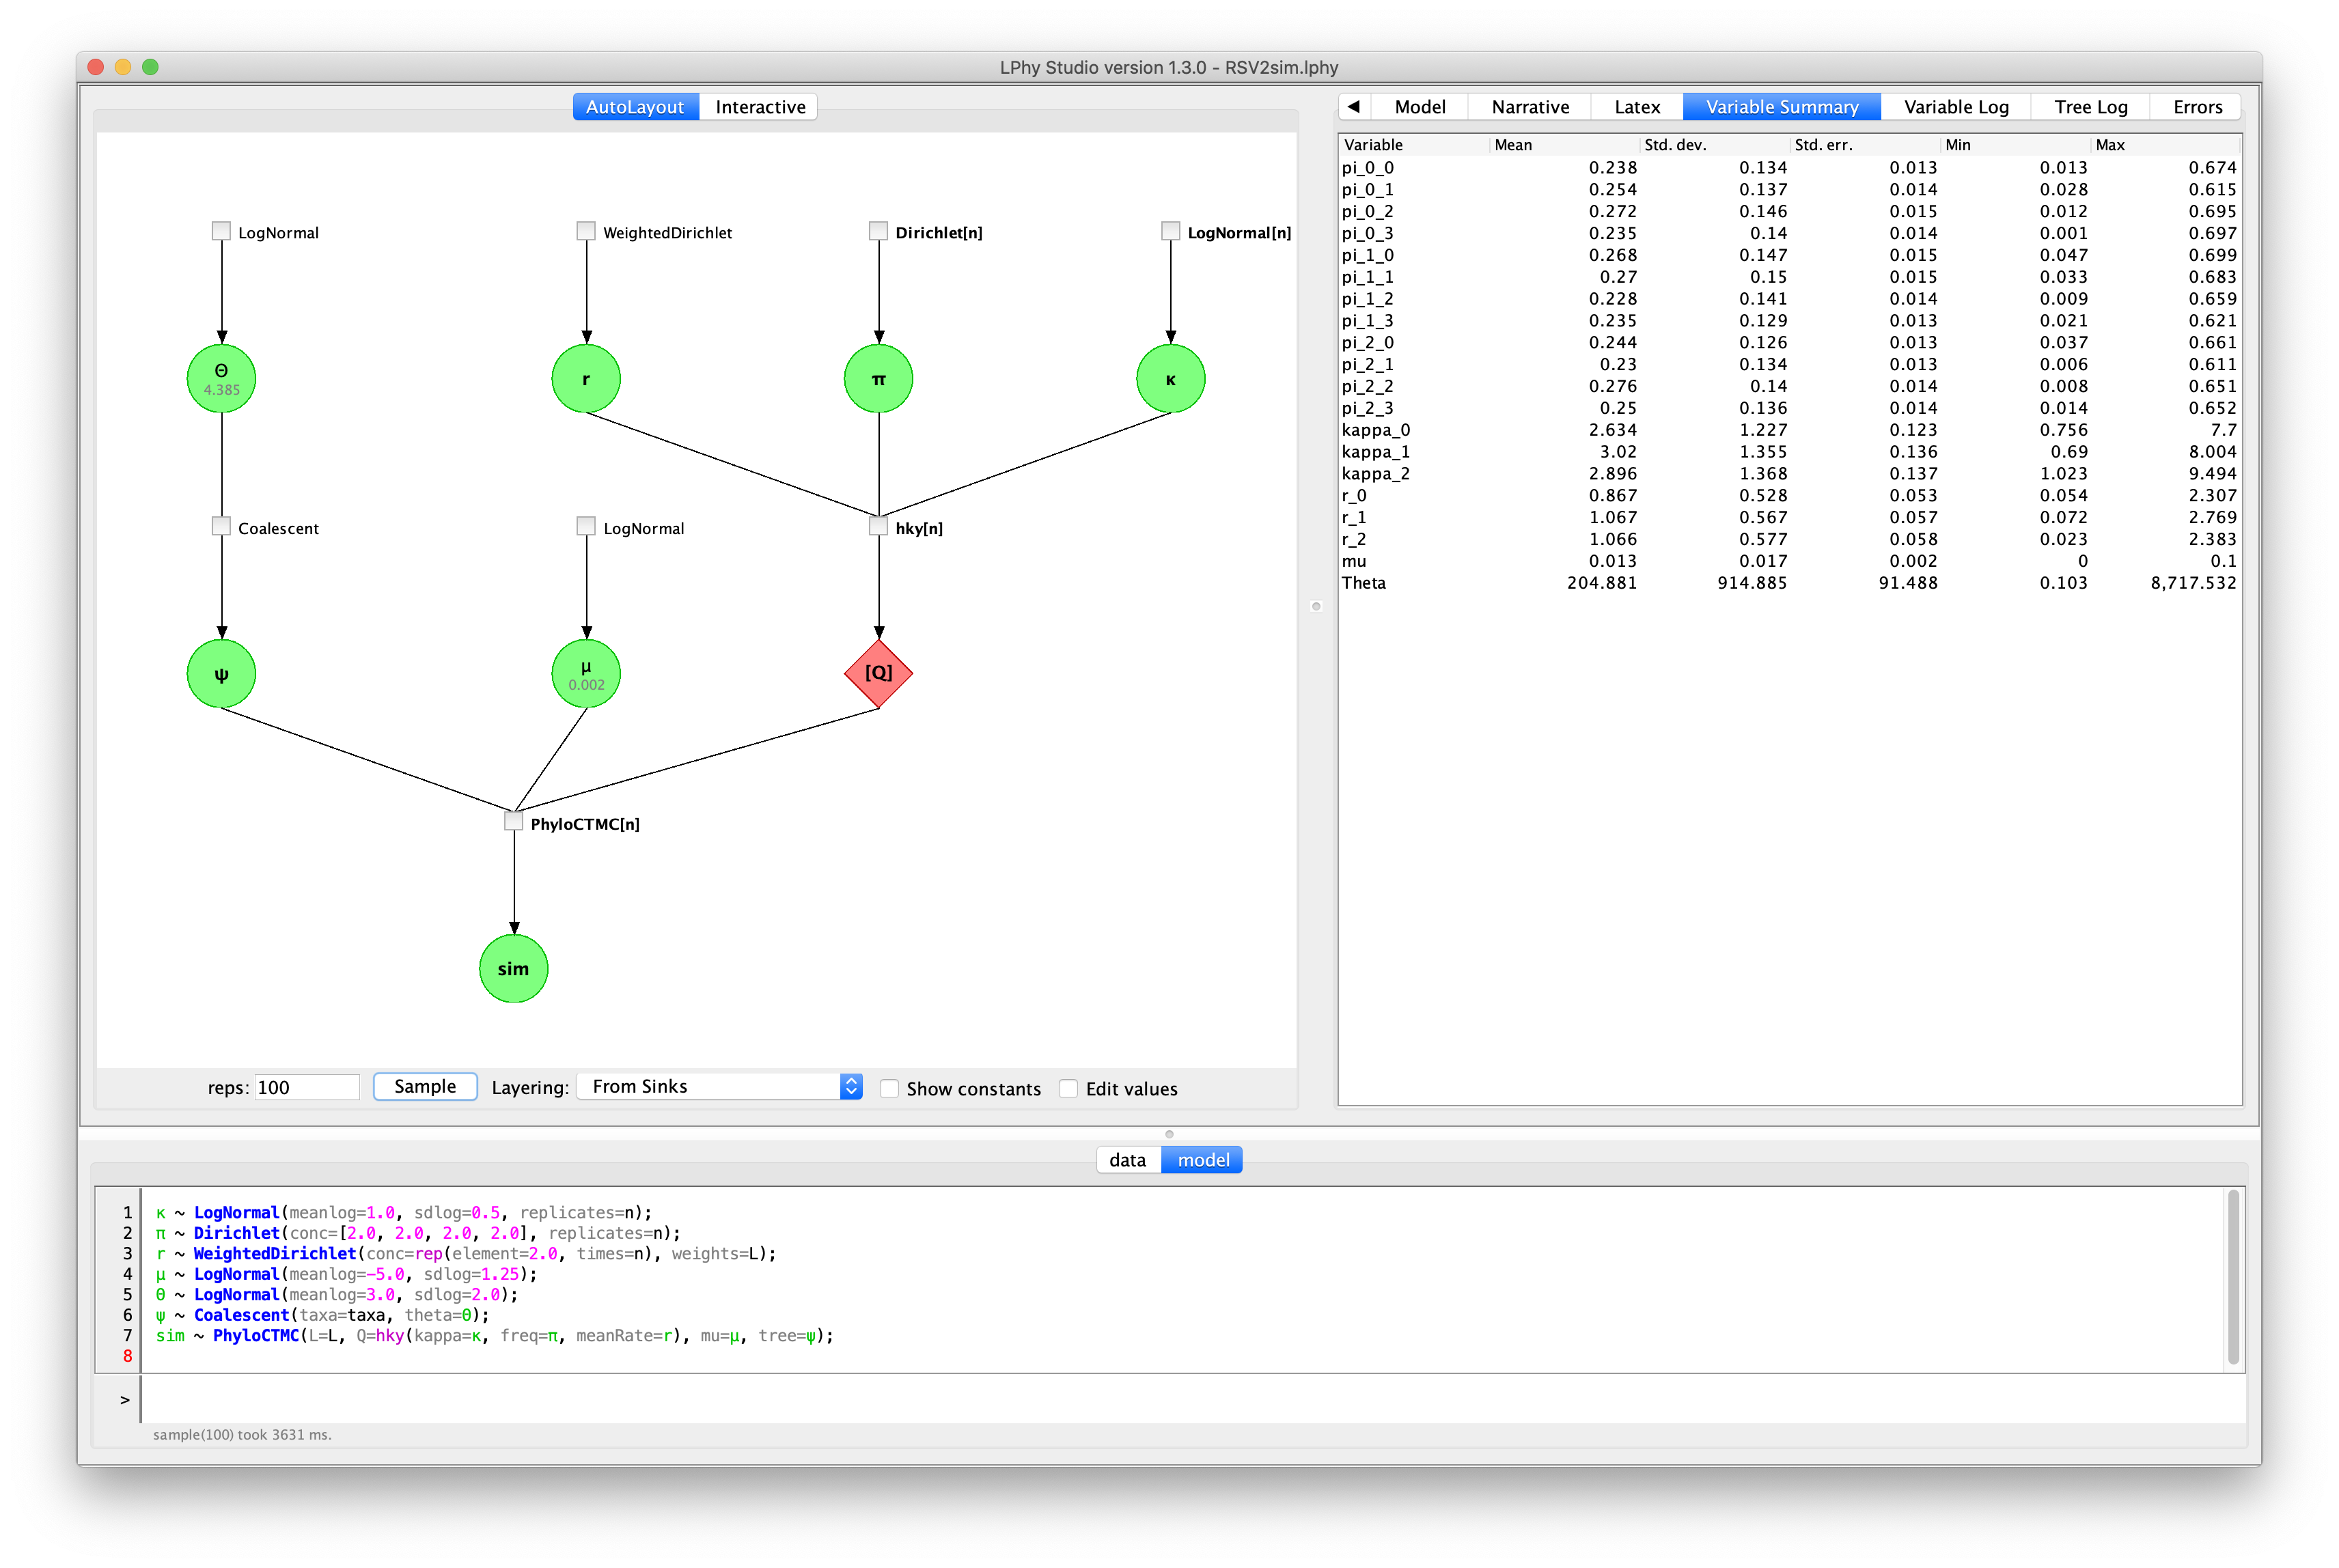
\includegraphics[width=\textwidth]{figs/simulations100.png}
%   \caption{A screenshot to run 100 simulations from the simple HKY+Coalescent model. The ``reps'' text field is used to define the number of simulations to run. The right panel shows the statistical summary of the simulated parameters.} 
%   \label{fig:simulations100}
% \end{figure}


\section*{Discussion}
Although there are many
programming languages through which statistical 
models can be succintly described (e.g., Stan
\cite{carpenter2017stan}, JAGS \cite{plummer2003jags}, BUGS
\cite{lunn2009bugs, gilks1994language}), these languages do not
support the unique feature of phylogenetic models: the phylogenetic
tree.
Phylogenetic trees are complex high-dimensional objects, part
discrete, part continuous.
There is no bijection between tree space and Euclidean space, so these
objects cannot be treated with standard statistical distributions \cite{gavryushkin2016space}.
Hence, specialist software is commonly employed to perform inference
involving phylogenetic trees
\cite{hohna2016revbayes,bouckaert2019beastanalysis}.

LinguaPhylo differs from existing specialist software in the way it handles model specification.
By using vectorization, LinguaPhylo obviates the need for for-loop control flow to describe repetitive structural elements of a model.
This feature lowers the risk of syntactic or programming logic mistakes when defining a model relative to a full programming language such as Rev \cite{revbayes}.
In its declarative nature, LPhy's language resembles the XML specification adopted by BEAST 2 \cite{bouckaert2014beast}, but shares the central notion of probabilistic graphical models with the Rev language.

LinguaPhylo provides for a form of array programming (vectorization), so that any function or
generative distribution can be called with its arguments in
vectorized form. In such situations the function or generative distribution is ``broadcast" over each element of the array (or indeed pairs or tuples of elements across multiple parallel arrays), which allows for very concise model descriptions.

%\textcolor{blue}{[FKM: More ideas for this section if we want to expand it a little -- (1) How and if LPhy is meant as a replacement for BEAUti, and if not, how it complements it, (2) Features BEAUti supports, but LPhy doesn't yet (and maybe will never support), like monophyletic constraints, node dating, (3) LPhy illuminates the model structure in a way BEAUti doesn't, (4) Taming the BEAST with LPhy? More community resources]}

Finally, future work on integration of LPhy with other popular Bayesian phylogenetic inference tools, such as BEAST \cite{suchard2018bayesian}, MrBayes\cite{ronquist2012mrbayes}, RevBayes\cite{hohna2016revbayes} will increase the flexibility of the framework, and enable easy validation of and comparison between different Bayesian phylogenetic inference engines.

\section*{Acknowledgments}
AJD was supported by a James Cook Fellowship. FKM was supported by Marsden grant 16-UOA-277 and by National Science Foundation grant DEB-2040347. We thank the New Zealand eScience Infrastructure (NeSI) for access to high-performance computation resources.

\nolinenumbers

% Either type in your references using
% \begin{thebibliography}{}
% \bibitem{}
% Text
% \end{thebibliography}
%
% or
%
% Compile your BiBTeX database using our plos2015.bst
% style file and paste the contents of your .bbl file
% here. See http://journals.plos.org/plosone/s/latex for 
% step-by-step instructions.
% 
\bibliography{linguaPhylo}



\end{document}
